% MCQMC 2022 article on the Challenges of Great MCQMC Software
%
% sample root file for your "contribution" to a contributed volume
%
% Use this file as a template for your own input.
%
%%%%%%%%%%%%%%%% Springer %%%%%%%%%%%%%%%%%%%%%%%%%%%%%%%%%%
%%%%%%%%%%%%%%%%%%%% author.tex %%%%%%%%%%%%%%%%%%%%%%%%%%%%%%%%%%%
%
% sample root file for your "contribution" to a contributed volume
%
% Use this file as a template for your own input.
%
%%%%%%%%%%%%%%%% Springer %%%%%%%%%%%%%%%%%%%%%%%%%%%%%%%%%%


% RECOMMENDED %%%%%%%%%%%%%%%%%%%%%%%%%%%%%%%%%%%%%%%%%%%%%%%%%%%
\documentclass[graybox]{svmult}

% choose options for [] as required from the list
% in the Reference Guide

\usepackage{type1cm}        % activate if the above 3 fonts are
% not available on your system
%
\usepackage{makeidx}         % allows index generation
\usepackage{graphicx}        % standard LaTeX graphics tool
% when including figure files
\usepackage{multicol}        % used for the two-column index
\usepackage[bottom]{footmisc}% places footnotes at page bottom


\usepackage{newtxtext}       %
\usepackage[varvw]{newtxmath}       % selects Times Roman as basic font

% see the list of further useful packages
% in the Reference Guide

%\makeindex             % used for the subject index
% please use the style svind.ist with
% your makeindex program

%%%%%%%%%%%%%%%%%%%%%%%%%%%%%%%%%%%%%%%%%%%%%%%%%%%%%%%%%%%%%%%%%%%%%%%%%%%%%%%%%%%%%%%%%

%%%%Fred start
%%%%
%% PLEASE NOTE: do not add anything to this file!!!
%% This file will not be used when processing your contribution
%%
%% You can use this file as a reference for commonly used packages 
%% and commonly defined macros, which we will enable by default for 
%% compiling the book.
%% If any of these clash with your own macros, then you will notice.
%% You are not allowed to redefine any of these...
%%%

%\RequirePackage[l2tabu,orthodox]{nag}

%\usepackage{mathptmx}       % selects Times Roman as basic font
%\usepackage{helvet}         % selects Helvetica as sans-serif font
%\usepackage{courier}        % selects Courier as typewriter font
%\usepackage{type1cm}       % activate if the above 3 fonts are
                            % not available on your system
\usepackage{graphicx}       % standard LaTeX graphics tool
                            % when including figure files

\usepackage[latin1]{inputenc}
\usepackage[T1]{fontenc}
\usepackage{microtype} % good font tricks

\usepackage{cite}
%\usepackage{url}
\usepackage{array,colortbl}
\usepackage{amsmath,amsfonts,bm,mathtools,mathrsfs} % taken out amssymb, amsthm

\DeclareFontFamily{U}{mathx}{\hyphenchar\font45}
\DeclareFontShape{U}{mathx}{m}{n}{
      <5> <6> <7> <8> <9> <10>
      <10.95> <12> <14.4> <17.28> <20.74> <24.88>
      mathx10
      }{}
\DeclareSymbolFont{mathx}{U}{mathx}{m}{n}
\DeclareFontSubstitution{U}{mathx}{m}{n}
\DeclareMathAccent{\widecheck}{0}{mathx}{"71}

% From: http://web.mit.edu/18.704/www/thmp2e.sty
%
% To facilitate putting citations in theorem/definition remarks,
%       \citep{pages}{source}
% is similar to
%       \cite[pages]{source}
% but lacks the square brackets, so that nested square brackets don't
% confuse LaTeX.
\def\citep#1#2{\cite[{#1}]{#2}}

% The followin are moved to common-macros.tex to be able to use this file with beamer which already defines some of the following:
%\theoremstyle{plain}
%  \newtheorem{theorem}{Theorem}
%  \newtheorem{proposition}{Proposition}
%  \newtheorem{lemma}{Lemma}
%  \newtheorem{corollary}{Corollary}
%  \newtheorem{alg}{Algorithm} % NB: there is also the algorithm environment from the algorithm package which is a floating environment
%  \newtheorem{assumption}{Assumption}
%\theoremstyle{definition}
%  \newtheorem{definition}{Definition}
%  \newtheorem{example}{Example}
%\theoremstyle{remark}
%  \newtheorem{remark}{Remark}

\newcommand{\RefEq}[1]{~\textup{(\ref{#1})}}
\newcommand{\RefEqTwo}[2]{~\textup{(\ref{#1})} and~\textup{(\ref{#2})}}
\newcommand{\RefDef}[1]{Definition~\textup{\ref{#1}}}
\newcommand{\RefSec}[1]{Section~\textup{\ref{#1}}}
\newcommand{\RefApp}[1]{Appendix~\textup{\ref{#1}}}
\newcommand{\RefThm}[1]{Theorem~\textup{\ref{#1}}}
\newcommand{\RefProp}[1]{Proposition~\textup{\ref{#1}}}
\newcommand{\RefLem}[1]{Lemma~\textup{\ref{#1}}}
\newcommand{\RefLemTwo}[2]{Lemmas~\textup{\ref{#1}} and~\textup{\ref{#2}}}
\newcommand{\RefCol}[1]{Corollary~\textup{\ref{#1}}}
\newcommand{\RefAlg}[1]{Algorithm~\textup{\ref{#1}}}
\newcommand{\RefFig}[1]{Figure~\textup{\ref{#1}}}
\newcommand{\RefFigTwo}[2]{Figures~\textup{\ref{#1}} and~\textup{\ref{#2}}}

\usepackage{algorithm}
\usepackage{algorithmic}
%\usepackage{algcompatible}
%\usepackage[compatible]{algpseudocode}
\renewcommand*{\thealgorithm}{\arabic{algorithm}}


% Note that Springer defines the following already:
%
% \D upright d for differential d
% \I upright i for imaginary unit
% \E upright e for exponential function
% \tens depicts tensors as sans serif upright
% \vec depicts vectors as boldface characters instead of the arrow accent
%
% Additionally we throw in the following common used macro's:

% blackboards:
% perl -e 'for $a ("A".."Z") { print "\\newcommand{\\bb$a}{{\\mathbb{$a}}}\n"; }'
\newcommand{\bbA}{{\mathbb{A}}}
\newcommand{\bbB}{{\mathbb{B}}}
\newcommand{\bbC}{{\mathbb{C}}}
\newcommand{\bbD}{{\mathbb{D}}}
\newcommand{\bbE}{{\mathbb{E}}}
\newcommand{\bbF}{{\mathbb{F}}}
\newcommand{\bbG}{{\mathbb{G}}}
\newcommand{\bbH}{{\mathbb{H}}}
\newcommand{\bbI}{{\mathbb{I}}}
\newcommand{\bbJ}{{\mathbb{J}}}
\newcommand{\bbK}{{\mathbb{K}}}
\newcommand{\bbL}{{\mathbb{L}}}
\newcommand{\bbM}{{\mathbb{M}}}
\newcommand{\bbN}{{\mathbb{N}}}
\newcommand{\bbO}{{\mathbb{O}}}
\newcommand{\bbP}{{\mathbb{P}}}
\newcommand{\bbQ}{{\mathbb{Q}}}
\newcommand{\bbR}{{\mathbb{R}}}
\newcommand{\bbS}{{\mathbb{S}}}
\newcommand{\bbT}{{\mathbb{T}}}
\newcommand{\bbU}{{\mathbb{U}}}
\newcommand{\bbV}{{\mathbb{V}}}
\newcommand{\bbW}{{\mathbb{W}}}
\newcommand{\bbX}{{\mathbb{X}}}
\newcommand{\bbY}{{\mathbb{Y}}}
\newcommand{\bbZ}{{\mathbb{Z}}}
% commonly used shortcuts:
\newcommand{\C}{{\mathbb{C}}} % complex numbers
\newcommand{\F}{{\mathbb{F}}} % field, finite field
\newcommand{\N}{{\mathbb{N}}} % natural numbers {1, 2, ...}
\newcommand{\Q}{{\mathbb{Q}}} % rationals
\newcommand{\R}{{\mathbb{R}}} % reals
\newcommand{\Z}{{\mathbb{Z}}} % integers
% more commonly used shortcuts:
\newcommand{\CC}{{\mathbb{C}}} % complex numbers
\newcommand{\FF}{{\mathbb{F}}} % field, finite field
\newcommand{\NN}{{\mathbb{N}}} % natural numbers {1, 2, ...}
\newcommand{\QQ}{{\mathbb{Q}}} % rationals
\newcommand{\RR}{{\mathbb{R}}} % reals
\newcommand{\ZZ}{{\mathbb{Z}}} % integers
% more commonly used shortcuts:
\newcommand{\EE}{{\mathbb{E}}}
\newcommand{\PP}{{\mathbb{P}}}
\newcommand{\TT}{{\mathbb{T}}}
\newcommand{\VV}{{\mathbb{V}}}
% and even more commonly used shortcuts:
\newcommand{\Complex}{{\mathbb{C}}}
\newcommand{\Integer}{{\mathbb{Z}}}
\newcommand{\Natural}{{\mathbb{N}}}
\newcommand{\Rational}{{\mathbb{Q}}}
\newcommand{\Real}{{\mathbb{R}}}
% indicator boldface 1:
%\DeclareSymbolFont{bbold}{U}{bbold}{m}{n}
%\DeclareSymbolFontAlphabet{\mathbbold}{bbold}
\newcommand{\ind}{{\mathbbold{1}}}
\newcommand{\bbone}{{\mathbbold{1}}}

% vectors as boldsymbols:
% perl -e 'for $a ("a".."z", "A".."Z") { print "\\newcommand{\\bs$a}{{\\boldsymbol{$a}}}\n"; }'
\newcommand{\bsa}{{\boldsymbol{a}}}
\newcommand{\bsb}{{\boldsymbol{b}}}
\newcommand{\bsc}{{\boldsymbol{c}}}
\newcommand{\bsd}{{\boldsymbol{d}}}
\newcommand{\bse}{{\boldsymbol{e}}}
\newcommand{\bsf}{{\boldsymbol{f}}}
\newcommand{\bsg}{{\boldsymbol{g}}}
\newcommand{\bsh}{{\boldsymbol{h}}}
\newcommand{\bsi}{{\boldsymbol{i}}}
\newcommand{\bsj}{{\boldsymbol{j}}}
\newcommand{\bsk}{{\boldsymbol{k}}}
\newcommand{\bsl}{{\boldsymbol{l}}}
\newcommand{\bsm}{{\boldsymbol{m}}}
\newcommand{\bsn}{{\boldsymbol{n}}}
\newcommand{\bso}{{\boldsymbol{o}}}
\newcommand{\bsp}{{\boldsymbol{p}}}
\newcommand{\bsq}{{\boldsymbol{q}}}
\newcommand{\bsr}{{\boldsymbol{r}}}
\newcommand{\bss}{{\boldsymbol{s}}}
\newcommand{\bst}{{\boldsymbol{t}}}
\newcommand{\bsu}{{\boldsymbol{u}}}
\newcommand{\bsv}{{\boldsymbol{v}}}
\newcommand{\bsw}{{\boldsymbol{w}}}
\newcommand{\bsx}{{\boldsymbol{x}}}
\newcommand{\bsy}{{\boldsymbol{y}}}
\newcommand{\bsz}{{\boldsymbol{z}}}
\newcommand{\bsA}{{\boldsymbol{A}}}
\newcommand{\bsB}{{\boldsymbol{B}}}
\newcommand{\bsC}{{\boldsymbol{C}}}
\newcommand{\bsD}{{\boldsymbol{D}}}
\newcommand{\bsE}{{\boldsymbol{E}}}
\newcommand{\bsF}{{\boldsymbol{F}}}
\newcommand{\bsG}{{\boldsymbol{G}}}
\newcommand{\bsH}{{\boldsymbol{H}}}
\newcommand{\bsI}{{\boldsymbol{I}}}
\newcommand{\bsJ}{{\boldsymbol{J}}}
\newcommand{\bsK}{{\boldsymbol{K}}}
\newcommand{\bsL}{{\boldsymbol{L}}}
\newcommand{\bsM}{{\boldsymbol{M}}}
\newcommand{\bsN}{{\boldsymbol{N}}}
\newcommand{\bsO}{{\boldsymbol{O}}}
\newcommand{\bsP}{{\boldsymbol{P}}}
\newcommand{\bsQ}{{\boldsymbol{Q}}}
\newcommand{\bsR}{{\boldsymbol{R}}}
\newcommand{\bsS}{{\boldsymbol{S}}}
\newcommand{\bsT}{{\boldsymbol{T}}}
\newcommand{\bsU}{{\boldsymbol{U}}}
\newcommand{\bsV}{{\boldsymbol{V}}}
\newcommand{\bsW}{{\boldsymbol{W}}}
\newcommand{\bsX}{{\boldsymbol{X}}}
\newcommand{\bsY}{{\boldsymbol{Y}}}
\newcommand{\bsZ}{{\boldsymbol{Z}}}
% other commonly used boldsymbols:
\newcommand{\bsell}{{\boldsymbol{\ell}}}
\newcommand{\bszero}{{\boldsymbol{0}}} % vector of zeros
\newcommand{\bsone}{{\boldsymbol{1}}}  % vector of ones
% boldsymbol greeks:
% perl -e 'for $a (qw(alpha beta gamma delta epsilon varepsilon zeta eta theta vartheta kappa lambda mu nu xi pi varpi rho varrho sigma varsigma tau upsilon phi varphi chi psi omega Gamma Delta Theta Lambda Xi Pi Sigma Upsilon Phi Psi Omega)) { print "\\newcommand{\\bs$a}{{\\boldsymbol{\\$a}}}\n"; }'
\newcommand{\bsalpha}{{\boldsymbol{\alpha}}}
\newcommand{\bsbeta}{{\boldsymbol{\beta}}}
\newcommand{\bsgamma}{{\boldsymbol{\gamma}}}
\newcommand{\bsdelta}{{\boldsymbol{\delta}}}
\newcommand{\bsepsilon}{{\boldsymbol{\epsilon}}}
\newcommand{\bsvarepsilon}{{\boldsymbol{\varepsilon}}}
\newcommand{\bszeta}{{\boldsymbol{\zeta}}}
\newcommand{\bseta}{{\boldsymbol{\eta}}}
\newcommand{\bstheta}{{\boldsymbol{\theta}}}
\newcommand{\bsvartheta}{{\boldsymbol{\vartheta}}}
\newcommand{\bskappa}{{\boldsymbol{\kappa}}}
\newcommand{\bslambda}{{\boldsymbol{\lambda}}}
\newcommand{\bsmu}{{\boldsymbol{\mu}}}
\newcommand{\bsnu}{{\boldsymbol{\nu}}}
\newcommand{\bsxi}{{\boldsymbol{\xi}}}
\newcommand{\bspi}{{\boldsymbol{\pi}}}
\newcommand{\bsvarpi}{{\boldsymbol{\varpi}}}
\newcommand{\bsrho}{{\boldsymbol{\rho}}}
\newcommand{\bsvarrho}{{\boldsymbol{\varrho}}}
\newcommand{\bssigma}{{\boldsymbol{\sigma}}}
\newcommand{\bsvarsigma}{{\boldsymbol{\varsigma}}}
\newcommand{\bstau}{{\boldsymbol{\tau}}}
\newcommand{\bsupsilon}{{\boldsymbol{\upsilon}}}
\newcommand{\bsphi}{{\boldsymbol{\phi}}}
\newcommand{\bsvarphi}{{\boldsymbol{\varphi}}}
\newcommand{\bschi}{{\boldsymbol{\chi}}}
\newcommand{\bspsi}{{\boldsymbol{\psi}}}
\newcommand{\bsomega}{{\boldsymbol{\omega}}}
\newcommand{\bsGamma}{{\boldsymbol{\Gamma}}}
\newcommand{\bsDelta}{{\boldsymbol{\Delta}}}
\newcommand{\bsTheta}{{\boldsymbol{\Theta}}}
\newcommand{\bsLambda}{{\boldsymbol{\Lambda}}}
\newcommand{\bsXi}{{\boldsymbol{\Xi}}}
\newcommand{\bsPi}{{\boldsymbol{\Pi}}}
\newcommand{\bsSigma}{{\boldsymbol{\Sigma}}}
\newcommand{\bsUpsilon}{{\boldsymbol{\Upsilon}}}
\newcommand{\bsPhi}{{\boldsymbol{\Phi}}}
\newcommand{\bsPsi}{{\boldsymbol{\Psi}}}
\newcommand{\bsOmega}{{\boldsymbol{\Omega}}}

% cals:
% perl -e 'for $a ("a".."z", "A".."Z") { print "\\newcommand{\\cal$a}{{\\mathcal{$a}}}\n"; }'
\newcommand{\cala}{{\mathcal{a}}}
\newcommand{\calb}{{\mathcal{b}}}
\newcommand{\calc}{{\mathcal{c}}}
\newcommand{\cald}{{\mathcal{d}}}
\newcommand{\cale}{{\mathcal{e}}}
\newcommand{\calf}{{\mathcal{f}}}
\newcommand{\calg}{{\mathcal{g}}}
\newcommand{\calh}{{\mathcal{h}}}
\newcommand{\cali}{{\mathcal{i}}}
\newcommand{\calj}{{\mathcal{j}}}
\newcommand{\calk}{{\mathcal{k}}}
\newcommand{\call}{{\mathcal{l}}}
\newcommand{\calm}{{\mathcal{m}}}
\newcommand{\caln}{{\mathcal{n}}}
\newcommand{\calo}{{\mathcal{o}}}
\newcommand{\calp}{{\mathcal{p}}}
\newcommand{\calq}{{\mathcal{q}}}
\newcommand{\calr}{{\mathcal{r}}}
\newcommand{\cals}{{\mathcal{s}}}
\newcommand{\calt}{{\mathcal{t}}}
\newcommand{\calu}{{\mathcal{u}}}
\newcommand{\calv}{{\mathcal{v}}}
\newcommand{\calw}{{\mathcal{w}}}
\newcommand{\calx}{{\mathcal{x}}}
\newcommand{\caly}{{\mathcal{y}}}
\newcommand{\calz}{{\mathcal{z}}}
\newcommand{\calA}{{\mathcal{A}}}
\newcommand{\calB}{{\mathcal{B}}}
\newcommand{\calC}{{\mathcal{C}}}
\newcommand{\calD}{{\mathcal{D}}}
\newcommand{\calE}{{\mathcal{E}}}
\newcommand{\calF}{{\mathcal{F}}}
\newcommand{\calG}{{\mathcal{G}}}
\newcommand{\calH}{{\mathcal{H}}}
\newcommand{\calI}{{\mathcal{I}}}
\newcommand{\calJ}{{\mathcal{J}}}
\newcommand{\calK}{{\mathcal{K}}}
\newcommand{\calL}{{\mathcal{L}}}
\newcommand{\calM}{{\mathcal{M}}}
\newcommand{\calN}{{\mathcal{N}}}
\newcommand{\calO}{{\mathcal{O}}}
\newcommand{\calP}{{\mathcal{P}}}
\newcommand{\calQ}{{\mathcal{Q}}}
\newcommand{\calR}{{\mathcal{R}}}
\newcommand{\calS}{{\mathcal{S}}}
\newcommand{\calT}{{\mathcal{T}}}
\newcommand{\calU}{{\mathcal{U}}}
\newcommand{\calV}{{\mathcal{V}}}
\newcommand{\calW}{{\mathcal{W}}}
\newcommand{\calX}{{\mathcal{X}}}
\newcommand{\calY}{{\mathcal{Y}}}
\newcommand{\calZ}{{\mathcal{Z}}}

% scrs:
% perl -e 'for $a ("a".."z", "A".."Z") { print "\\newcommand{\\scr$a}{{\\mathscr{$a}}}\n"; }'
\newcommand{\scra}{{\mathscr{a}}}
\newcommand{\scrb}{{\mathscr{b}}}
\newcommand{\scrc}{{\mathscr{c}}}
\newcommand{\scrd}{{\mathscr{d}}}
\newcommand{\scre}{{\mathscr{e}}}
\newcommand{\scrf}{{\mathscr{f}}}
\newcommand{\scrg}{{\mathscr{g}}}
\newcommand{\scrh}{{\mathscr{h}}}
\newcommand{\scri}{{\mathscr{i}}}
\newcommand{\scrj}{{\mathscr{j}}}
\newcommand{\scrk}{{\mathscr{k}}}
\newcommand{\scrl}{{\mathscr{l}}}
\newcommand{\scrm}{{\mathscr{m}}}
\newcommand{\scrn}{{\mathscr{n}}}
\newcommand{\scro}{{\mathscr{o}}}
\newcommand{\scrp}{{\mathscr{p}}}
\newcommand{\scrq}{{\mathscr{q}}}
\newcommand{\scrr}{{\mathscr{r}}}
\newcommand{\scrs}{{\mathscr{s}}}
\newcommand{\scrt}{{\mathscr{t}}}
\newcommand{\scru}{{\mathscr{u}}}
\newcommand{\scrv}{{\mathscr{v}}}
\newcommand{\scrw}{{\mathscr{w}}}
\newcommand{\scrx}{{\mathscr{x}}}
\newcommand{\scry}{{\mathscr{y}}}
\newcommand{\scrz}{{\mathscr{z}}}
\newcommand{\scrA}{{\mathscr{A}}}
\newcommand{\scrB}{{\mathscr{B}}}
\newcommand{\scrC}{{\mathscr{C}}}
\newcommand{\scrD}{{\mathscr{D}}}
\newcommand{\scrE}{{\mathscr{E}}}
\newcommand{\scrF}{{\mathscr{F}}}
\newcommand{\scrG}{{\mathscr{G}}}
\newcommand{\scrH}{{\mathscr{H}}}
\newcommand{\scrI}{{\mathscr{I}}}
\newcommand{\scrJ}{{\mathscr{J}}}
\newcommand{\scrK}{{\mathscr{K}}}
\newcommand{\scrL}{{\mathscr{L}}}
\newcommand{\scrM}{{\mathscr{M}}}
\newcommand{\scrN}{{\mathscr{N}}}
\newcommand{\scrO}{{\mathscr{O}}}
\newcommand{\scrP}{{\mathscr{P}}}
\newcommand{\scrQ}{{\mathscr{Q}}}
\newcommand{\scrR}{{\mathscr{R}}}
\newcommand{\scrS}{{\mathscr{S}}}
\newcommand{\scrT}{{\mathscr{T}}}
\newcommand{\scrU}{{\mathscr{U}}}
\newcommand{\scrV}{{\mathscr{V}}}
\newcommand{\scrW}{{\mathscr{W}}}
\newcommand{\scrX}{{\mathscr{X}}}
\newcommand{\scrY}{{\mathscr{Y}}}
\newcommand{\scrZ}{{\mathscr{Z}}}

% Euler fraks:
% perl -e 'for $a ("a".."z", "A".."Z") { print "\\newcommand{\\frak$a}{{\\mathfrak{$a}}}\n"; }'
\newcommand{\fraka}{{\mathfrak{a}}}
\newcommand{\frakb}{{\mathfrak{b}}}
\newcommand{\frakc}{{\mathfrak{c}}}
\newcommand{\frakd}{{\mathfrak{d}}}
\newcommand{\frake}{{\mathfrak{e}}}
\newcommand{\frakf}{{\mathfrak{f}}}
\newcommand{\frakg}{{\mathfrak{g}}}
\newcommand{\frakh}{{\mathfrak{h}}}
\newcommand{\fraki}{{\mathfrak{i}}}
\newcommand{\frakj}{{\mathfrak{j}}}
\newcommand{\frakk}{{\mathfrak{k}}}
\newcommand{\frakl}{{\mathfrak{l}}}
\newcommand{\frakm}{{\mathfrak{m}}}
\newcommand{\frakn}{{\mathfrak{n}}}
\newcommand{\frako}{{\mathfrak{o}}}
\newcommand{\frakp}{{\mathfrak{p}}}
\newcommand{\frakq}{{\mathfrak{q}}}
\newcommand{\frakr}{{\mathfrak{r}}}
\newcommand{\fraks}{{\mathfrak{s}}}
\newcommand{\frakt}{{\mathfrak{t}}}
\newcommand{\fraku}{{\mathfrak{u}}}
\newcommand{\frakv}{{\mathfrak{v}}}
\newcommand{\frakw}{{\mathfrak{w}}}
\newcommand{\frakx}{{\mathfrak{x}}}
\newcommand{\fraky}{{\mathfrak{y}}}
\newcommand{\frakz}{{\mathfrak{z}}}
\newcommand{\frakA}{{\mathfrak{A}}}
\newcommand{\frakB}{{\mathfrak{B}}}
\newcommand{\frakC}{{\mathfrak{C}}}
\newcommand{\frakD}{{\mathfrak{D}}}
\newcommand{\frakE}{{\mathfrak{E}}}
\newcommand{\frakF}{{\mathfrak{F}}}
\newcommand{\frakG}{{\mathfrak{G}}}
\newcommand{\frakH}{{\mathfrak{H}}}
\newcommand{\frakI}{{\mathfrak{I}}}
\newcommand{\frakJ}{{\mathfrak{J}}}
\newcommand{\frakK}{{\mathfrak{K}}}
\newcommand{\frakL}{{\mathfrak{L}}}
\newcommand{\frakM}{{\mathfrak{M}}}
\newcommand{\frakN}{{\mathfrak{N}}}
\newcommand{\frakO}{{\mathfrak{O}}}
\newcommand{\frakP}{{\mathfrak{P}}}
\newcommand{\frakQ}{{\mathfrak{Q}}}
\newcommand{\frakR}{{\mathfrak{R}}}
\newcommand{\frakS}{{\mathfrak{S}}}
\newcommand{\frakT}{{\mathfrak{T}}}
\newcommand{\frakU}{{\mathfrak{U}}}
\newcommand{\frakV}{{\mathfrak{V}}}
\newcommand{\frakW}{{\mathfrak{W}}}
\newcommand{\frakX}{{\mathfrak{X}}}
\newcommand{\frakY}{{\mathfrak{Y}}}
\newcommand{\frakZ}{{\mathfrak{Z}}}
% sets as Euler fraks:
% perl -e 'for $a ("a".."z", "A".."Z") { print "\\newcommand{\\set$a}{{\\mathfrak{$a}}}\n"; }'
\newcommand{\seta}{{\mathfrak{a}}}
\newcommand{\setb}{{\mathfrak{b}}}
\newcommand{\setc}{{\mathfrak{c}}}
\newcommand{\setd}{{\mathfrak{d}}}
\newcommand{\sete}{{\mathfrak{e}}}
\newcommand{\setf}{{\mathfrak{f}}}
\newcommand{\setg}{{\mathfrak{g}}}
\newcommand{\seth}{{\mathfrak{h}}}
\newcommand{\seti}{{\mathfrak{i}}}
\newcommand{\setj}{{\mathfrak{j}}}
\newcommand{\setk}{{\mathfrak{k}}}
\newcommand{\setl}{{\mathfrak{l}}}
\newcommand{\setm}{{\mathfrak{m}}}
\newcommand{\setn}{{\mathfrak{n}}}
\newcommand{\seto}{{\mathfrak{o}}}
\newcommand{\setp}{{\mathfrak{p}}}
\newcommand{\setq}{{\mathfrak{q}}}
\newcommand{\setr}{{\mathfrak{r}}}
\newcommand{\sets}{{\mathfrak{s}}}
\newcommand{\sett}{{\mathfrak{t}}}
\newcommand{\setu}{{\mathfrak{u}}}
\newcommand{\setv}{{\mathfrak{v}}}
\newcommand{\setw}{{\mathfrak{w}}}
\newcommand{\setx}{{\mathfrak{x}}}
\newcommand{\sety}{{\mathfrak{y}}}
\newcommand{\setz}{{\mathfrak{z}}}
\newcommand{\setA}{{\mathfrak{A}}}
\newcommand{\setB}{{\mathfrak{B}}}
\newcommand{\setC}{{\mathfrak{C}}}
\newcommand{\setD}{{\mathfrak{D}}}
\newcommand{\setE}{{\mathfrak{E}}}
\newcommand{\setF}{{\mathfrak{F}}}
\newcommand{\setG}{{\mathfrak{G}}}
\newcommand{\setH}{{\mathfrak{H}}}
\newcommand{\setI}{{\mathfrak{I}}}
\newcommand{\setJ}{{\mathfrak{J}}}
\newcommand{\setK}{{\mathfrak{K}}}
\newcommand{\setL}{{\mathfrak{L}}}
\newcommand{\setM}{{\mathfrak{M}}}
\newcommand{\setN}{{\mathfrak{N}}}
\newcommand{\setO}{{\mathfrak{O}}}
\newcommand{\setP}{{\mathfrak{P}}}
\newcommand{\setQ}{{\mathfrak{Q}}}
\newcommand{\setR}{{\mathfrak{R}}}
\newcommand{\setS}{{\mathfrak{S}}}
\newcommand{\setT}{{\mathfrak{T}}}
\newcommand{\setU}{{\mathfrak{U}}}
\newcommand{\setV}{{\mathfrak{V}}}
\newcommand{\setW}{{\mathfrak{W}}}
\newcommand{\setX}{{\mathfrak{X}}}
\newcommand{\setY}{{\mathfrak{Y}}}
\newcommand{\setZ}{{\mathfrak{Z}}}

% math roman 
% perl -e 'for $a ("a".."z", "A".."Z") { print "\\newcommand{\\rm$a}{{\\mathrm{$a}}}\n"; }'
\newcommand{\rma}{{\mathrm{a}}}
\newcommand{\rmb}{{\mathrm{b}}}
\newcommand{\rmc}{{\mathrm{c}}}
\newcommand{\rmd}{{\mathrm{d}}}
\newcommand{\rme}{{\mathrm{e}}}
\newcommand{\rmf}{{\mathrm{f}}}
\newcommand{\rmg}{{\mathrm{g}}}
\newcommand{\rmh}{{\mathrm{h}}}
\newcommand{\rmi}{{\mathrm{i}}}
\newcommand{\rmj}{{\mathrm{j}}}
\newcommand{\rmk}{{\mathrm{k}}}
\newcommand{\rml}{{\mathrm{l}}}
\newcommand{\rmm}{{\mathrm{m}}}
\newcommand{\rmn}{{\mathrm{n}}}
\newcommand{\rmo}{{\mathrm{o}}}
\newcommand{\rmp}{{\mathrm{p}}}
\newcommand{\rmq}{{\mathrm{q}}}
\newcommand{\rmr}{{\mathrm{r}}}
\newcommand{\rms}{{\mathrm{s}}}
\newcommand{\rmt}{{\mathrm{t}}}
\newcommand{\rmu}{{\mathrm{u}}}
\newcommand{\rmv}{{\mathrm{v}}}
\newcommand{\rmw}{{\mathrm{w}}}
\newcommand{\rmx}{{\mathrm{x}}}
\newcommand{\rmy}{{\mathrm{y}}}
\newcommand{\rmz}{{\mathrm{z}}}
\newcommand{\rmA}{{\mathrm{A}}}
\newcommand{\rmB}{{\mathrm{B}}}
\newcommand{\rmC}{{\mathrm{C}}}
\newcommand{\rmD}{{\mathrm{D}}}
\newcommand{\rmE}{{\mathrm{E}}}
\newcommand{\rmF}{{\mathrm{F}}}
\newcommand{\rmG}{{\mathrm{G}}}
\newcommand{\rmH}{{\mathrm{H}}}
\newcommand{\rmI}{{\mathrm{I}}}
\newcommand{\rmJ}{{\mathrm{J}}}
\newcommand{\rmK}{{\mathrm{K}}}
\newcommand{\rmL}{{\mathrm{L}}}
\newcommand{\rmM}{{\mathrm{M}}}
\newcommand{\rmN}{{\mathrm{N}}}
\newcommand{\rmO}{{\mathrm{O}}}
\newcommand{\rmP}{{\mathrm{P}}}
\newcommand{\rmQ}{{\mathrm{Q}}}
\newcommand{\rmR}{{\mathrm{R}}}
\newcommand{\rmS}{{\mathrm{S}}}
\newcommand{\rmT}{{\mathrm{T}}}
\newcommand{\rmU}{{\mathrm{U}}}
\newcommand{\rmV}{{\mathrm{V}}}
\newcommand{\rmW}{{\mathrm{W}}}
\newcommand{\rmX}{{\mathrm{X}}}
\newcommand{\rmY}{{\mathrm{Y}}}
\newcommand{\rmZ}{{\mathrm{Z}}}

% other commons:
\newcommand{\wal}{{\rm wal}}
\newcommand{\icomp}{\mathrm{i}}
\newcommand{\abs}[1]{\left\vert#1\right\vert}
\newcommand{\norm}[1]{\left\Vert#1\right\Vert}
\newcommand{\floor}[1]{\left\lfloor #1 \right\rfloor} % floor
\newcommand{\ceil}[1]{\left\lceil #1 \right\rceil}    % ceil
\newcommand{\rd}{\,\mathrm{d}} % differential symbol with tiny space in front for use in integrals
\newcommand{\rdd}{\mathrm{d}} % differential symbol without space
\DeclareMathOperator{\cov}{Cov}
\DeclareMathOperator{\var}{Var}
\providecommand{\argmin}{\operatorname*{argmin}}
\providecommand{\argmax}{\operatorname*{argmax}}
\newcommand{\mcol}{{\mathpunct{:}}}


\usepackage{cite}
\usepackage{xspace}
\usepackage[hyphens]{url}
\providecommand{\HickernellFJ}{Hickernell\xspace}
\graphicspath{{ProgramsImages/}}

%\input FJHDef.tex
\newcommand{\AGSComment}[1]{{\color{red} #1}}

%%%%Fred end

\begin{document}

\title*{Challenges in Developing Great Quasi-Monte Carlo Software}
\authorrunning{S.-C.\ T.\ Choi et al}
\author{Sou-Cheng Terrya Choi \and Yuhan Ding \and Fred J. Hickernell \and R. Jagadeeswaran Aleksei G. Sorokin}
\institute{
Sou-Cheng Terrya Choi \at Department of Applied Mathematics, Illinois Institute of Technology,\\ RE 220, 10 W.\ 32$^{\text{nd}}$ St., Chicago, IL 60616 \email{schoi32@hawk.iit.edu}
\and
Yuhan Ding \at
 Department of Applied Mathematics, Illinois Institute of Technology,\\ RE 220, 10 W.\ 32$^{\text{nd}}$ St., Chicago, IL 60616 \email{yding2@hawk.iit.edu}
\and
Fred J. Hickernell \at Center for Interdisciplinary Scientific Computation and \\
Department of Applied Mathematics, Illinois Institute of Technology \\ RE 220, 10 W.\ 32$^{\text{nd}}$ St., Chicago, IL 60616 \email{hickernell@iit.edu}
\and
R. Jagadeeswaran \at
Department of Applied Mathematics, Illinois Institute of Technology,\\ RE 220, 10 W.\ 32$^{\text{nd}}$ St., Chicago, IL 60616 \email{jrathin1@hawk.iit.edu}
\and
Aleksei G. Sorokin \at
Department of Applied Mathematics, Illinois Institute of Technology,\\ RE 220, 10 W.\ 32$^{\text{nd}}$ St., Chicago, IL 60616 \email{asorokin@hawk.iit.edu}}

\maketitle

\abstract{
Quasi-Monte Carlo (QMC) methods have developed over several decades. With the explosion in computational science, there is a need for great software to realize that implements QMC algorithms. We review what QMC software has been developed to date, propose some criteria for developing great QMC software, and suggest some steps toward achieving great software.
}


\section{Introduction}

A QMC approximation of $\mu := \EE[f(\bsX)]$, $\bsX \sim \calU[0,1]^d$ can be implemented in a few steps:
\begin{enumerate}
    \item Draw a sequence of $n$ a low discrepancy (LD) \cite{Nie92, SloJoe94, DicEtal14a, DicEtal22a} nodes,
    $\bsx_1,\dots,\bsx_n$ that mimic $\calU[0,1]^d$.
    \item Evaluate the integrand $f$ at these nodes to obtain $f(\bsx_i)$, $i=1,\dots,n$.
    \item Estimate the true mean, $\mu$, by the sample mean
    \begin{equation}
        \hat{\mu} := \frac{1}{n} \sum_{i=1}^n f(\bsx_i).
        \label{eq:mc_average}
    \end{equation}
\end{enumerate}
However, the practice of QMC is often more complicated.  The original problem may need to be rewritten to fit above form and/or to facilitate a good approximation with small $n$.  Practitioners may wish to determine $n$ adaptively to satisfy a prescribed error tolerance.

In the next section we describe why QMC software is important.  We then discuss characteristics of great QMC software:

\begin{itemize}
\item Integrated with related libraries (Sect.\ \ref{CDHJS_sec:integrated}),

\item Correct (Sect.\ \ref{CDHJS_sec:correct}),

\item Efficient in computational time and memory (Sect.\ \ref{CDHJS_sec:efficient}),

\item Accessible to practitioners and theorists alike (Sect.\ \ref{CDHJS_sec:accessible}), and

\item Sustainable by a community that owns it (Sect.\ \ref{CDHJS_sec:sustainable}).

\end{itemize}

In each section we describe the challenges faced and how they might be overcome.



\section{Why Develop QMC Software} \label{CDHJS_sec:why_we_need_software}

Recent interest in quality scientific software is exemplified by the 2021 US Department of Energy \emph{Workshop on the Science of Scientific-Software Development and Use} \cite{ASCR-SSSDU,osti_1846008}. This workshop not only discussed diagnostics and treatments for the challenges of developing great scientific software, but also emphasized the importance of implementing theoretical advancements into well written, accessible software libraries. Three cross-cutting themes that arose in this workshop were
\begin{itemize}
    \item  We need to consider both human and technical elements to better understand how to improve the development and use of scientific software.

    \item We need to address urgent challenges in workforce recruitment and retention in the computing sciences with growth through expanded diversity, stable career paths, and the creation of a community and culture that attract and retain new generations of scientists.

    \item Scientific software has become essential to all areas of science and technology, creating opportunities for expanded partnerships, collaboration, and impact.
\end{itemize}
These themes apply to QMC software in particular, as well as scientific software in general.

\subsection{QMC Theory to Software}

QMC software makes theoretical advances in QMC available to practitioners. However, translating pseudo-code into good executable code is nuanced.  Software developers must write code that is computationally efficient, numerical stable, and provides reasonable default choices of tuning parameters. Great QMC software relieves users of these concerns.

\subsection{QMC Software to Theory}

Great QMC software opens up new application areas for QMC methods by allowing practitioners to compare new methods to existing ones.  QMC software has been successful in quantitative finance, uncertainty quantification, and image rendering. Unexpectedly good or bad computational results leads to open theoretical questions.  For example, the early application of QMC to high dimensional integrals arising in financial risk \cite{PasTra95} led to a wave of theoretical results on the tractability of integration in weighted spaces \cite{Woz99a,DicEtal14a,NovWoz10a}.

We next discuss characteristics of great QMC software outlined in the introduction.  For each characteristic we identify what is lacking and what might be done to remedy the lack.

\section{Integrated} \label{CDHJS_sec:integrated}

Expanding on the problem formulation in the introduction, we want to approximate well the integral or expectation, $\mu$, by the sample mean, $\hat{\mu}$:
\begin{gather}
\label{eq:cubSummary}
	\mu : = \int_\calT g(\bst) \, \lambda(\bst) \, \D \bst  = \bbE[f(\bsX)] = \int_{[0,1]^d} f(\bsx)  \, \D \bsx \approx \frac 1n \sum_{i=0}^{n-1} f(\bsx_i) =: \hat{\mu}_n, \\
 \label{CDHJS_eq:error_tol}
 \abs{\mu - \hat{\mu}_n} \le \varepsilon.
\end{gather}
Progressing from the original problem to a satisfactory solution requires several software components, which we describe in the subsections below.  Great QMC software environments allows different implementations of these components to be freely interchanged.

\subsection{LD Sequence Generators} A lattice, digital sequence, or Halton sequence generator typically supplies the sequence $\bsx_1, \bsx_2, \ldots$.  These sequences may be deterministic or random and are intended to have an empirical distribution that approximates well the uniform distribution.

LD generators are the most prevalent generally available components of QMC software.  These generators appear in Association of Computing Machinery  publications \cite{BraFox88,BraFoxNie92,HonHic00a}, FinDer \cite{PasTra95,FinDer}, libseq \cite{FriKel02,FriKelweb}, BRODA \cite{BRODA20a}, NAG \cite{NAG27}, MATLAB \cite{MAT9.13}, SamplePack \cite{SamplePack}, Gr\"unschlo{\ss}'s website \cite{GruWeb}, the Magic Point Shop \cite{NuyWeb}, R \cite{QRNG2020}, Julia \cite{QMCJulia}, PyTorch \cite{paszke2019pytorch}, SAS \cite{SAS_LD}, SciPy \cite{virtanen2020scipy}, and TensorFlow \cite{tfqfQMC2021a}, MatBuilder \cite{paulin2022}, and  QMCPy \cite{QMCPy2020a}.

Lattice and digital sequences are not unique, and improved or alternative versions continue to be constructed.  Joe and Kuo \cite{JoeKuo03,JoeKuo08,SobolDirection} have proposed  Sobol' generator direction numbers, which are now widely used, but were not part of the early LD sequence software.  L'Ecuyer and colleagues have created LatNetBuilder \cite{LatNet} to construct good lattice and polynomial lattice sequences based on user defined criteria. As was raised during a lunch at MCQMC 2022, we should agree on a consistent format for storing the parameters that define good LD sequences so that they can by shared across software libraries.

Users computing solutions in comprehensive software environments, such as NAG, MATLAB, R, SciPy, and TensorFlow, have convenient access to LD sequence generators.  However, most of these could provide more flexibility in their LD offerings.  Some large environments, such as  Dakota \cite{DakotaUsersManual} and SAS, have quite limited LD generators and should expand their offerings.  Developers of smaller libraries with more QMC features, like BRODA and QMCPy, should demonstrate how their libraries can connect well with other software environments.  An example involving QMCPy is given in the next subsection.

\subsection{Integrands and Variable Transformations} \label{CDHJS:sec:integrands}
The original integral or expectation arising from the application is defined in terms of the integrand, $g$, and the non-negative weight, $\lambda$.  For example,
\begin{itemize}
	\item $g$ is the discounted payoff of a financial derivative and $\lambda$ is the probability density function (PDF) for a discretized Brownian motion \cite{Gla03},

	\item  $g$ is the velocity of a fluid at a point in rock with a random porosity field whose discretized PDF is $\lambda$ \cite{KuoNuy16a}, or

	\item $g\lambda$ is the unnormalized Bayesian posterior density multiplied by parameter of interest \cite{GelEtal13}.
\end{itemize}

To put $\mu$ into the form that is directly accessible to QMC methods requires a variable transformation, $\bsPsi$, such that
\begin{equation*}
    \Psi((0,1)^d) = \calT, \qquad f(\bsx) = g(\bsPsi(\bsx)) \lambda(\bsPsi(\bsx)) \abs{\frac{\partial \bsPsi}{\partial\bsx}}.
\end{equation*}
Such a transformation is typically non-unique, and the choice of a good one is equivalent to importance sampling.  If $\lambda$ is a PDF for a random variable $\bsT$, then $\mu = \EE[g(\bsT)]$.  Moreover, one might choose $\bsPsi$ such that $\bsT = \bsPsi(\bsX)$, in which case $\lambda(\bsPsi(\bsx)) \abs{\partial \bsPsi/\partial\bsx} = 1$ and $f(\bsx) = g(\bsPsi(\bsx))$.

\begin{figure}
    \centering
    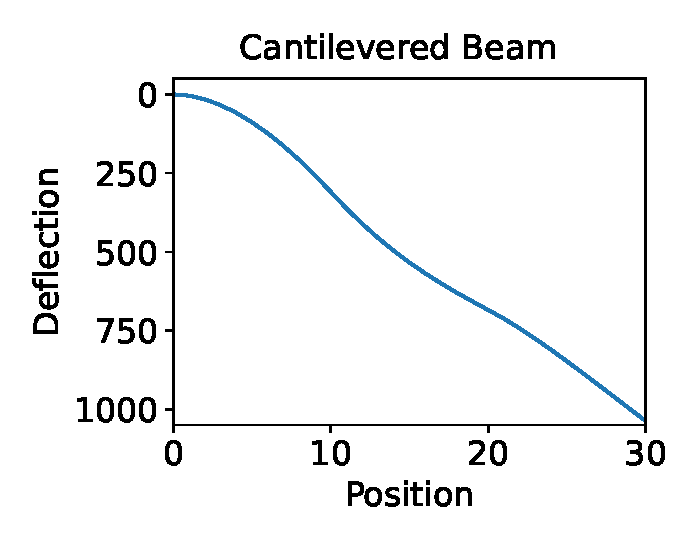
\includegraphics[width=0.5\textwidth]{cantileveredbeamwords.eps}
    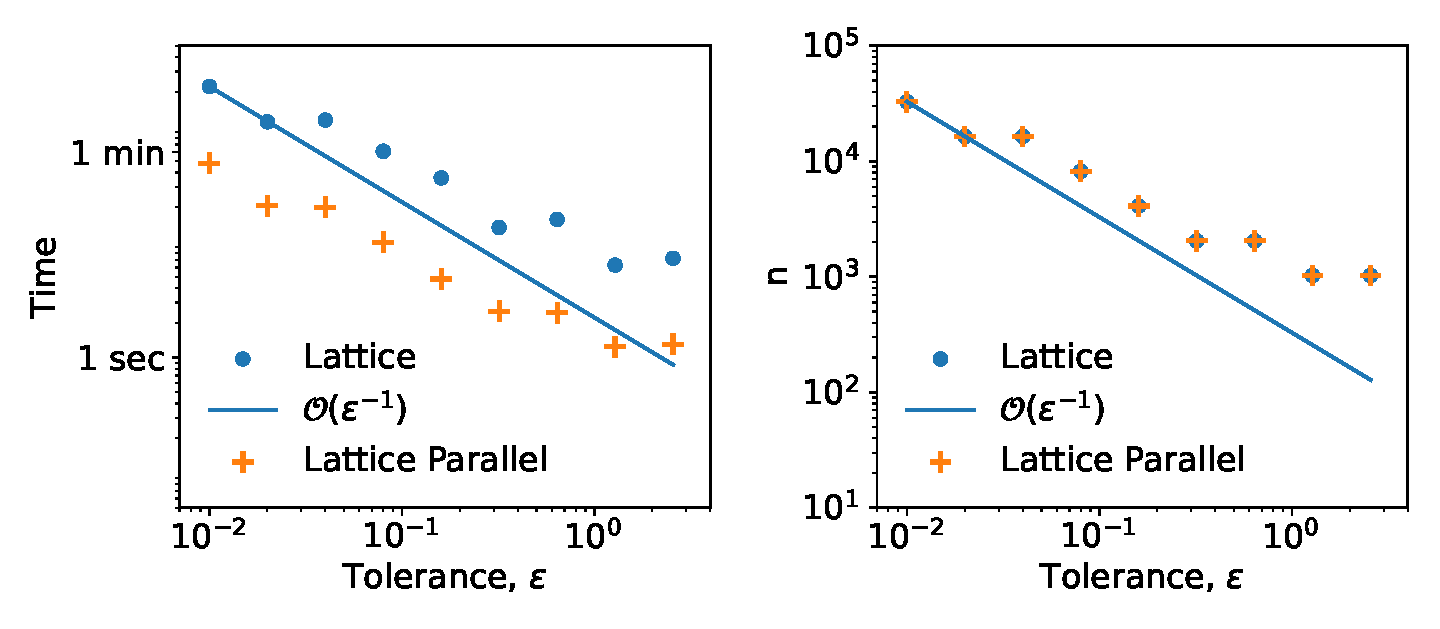
\includegraphics[width=0.7\textwidth]{ldparallelbeam.eps}
    \caption{The expected deflection of a beam with random Young's modulus.  QMCPy computes the answer in serial and in parallel using UM-Bridge and docker containers.  For small error tolerances, the time and sample size is $\calO(n^{-1})$, and parallel processing gives a speed-up of factor four to five.}
    \label{fig:beam}
\end{figure}

Complex integrands might be best evaluated by libraries that have no direct connection to QMC software libraries.  In the uncertainty quantification (UQ) space, the recently developed UQ and Model Bridge (UM-Bridge) \cite{umbridge}, connects libraries that generate sequences of model parameters, $\bsx_1, \bsx_2, \ldots$ with libraries that evaluate models, $f(\bsx_1), f(\bsx_2), \ldots$.  We illustrate in Figure \ref{fig:beam} how UM-Bridge connects QMCPy with a differential equation boundary value problem solver for a cantilevered beam with random Young's modulus \cite{ParSee22a}, where the randomness is given by $\bsX \sim \calU[1,1.2]^3$.  The beam position is discretized at $31$ points.  QMCPy computes the expected deflection of the beam a these points for a sequence of error tolerances using lattice rules.  By taking advantage of virtual machines and docker containers, the evaluation of the beam deflection can be computed in parallel in multiple cores of a single CPU to decrease execution time.

We need more connections of QMC software to other libraries, like what has been done with  QMCPy with and UM-Bridge.  This will facilitate allow newer and better QMC algorithms to tackle new applications.

\subsection{Stopping Criteria}
The cantilevered beam example illustrated in Figure \ref{fig:beam} utilizes QMCPy's stopping criterion to choose the sample size, $n$, based on the input error tolerance, $\varepsilon$, and the observed discrete Fourier series coefficients of the integrand, $f$.  See \cite{HicJim16a} for details of this stopping criterion for lattice rules.  Theoretically justified stopping criteria for choosing sample sizes are important and a relatively recent development \cite{HicEtal14a,HicJim16a,JimHic16a,RatHic19a,JagHic22a}.  Some of these stopping criteria for absolute error criteria, \eqref{CDHJS_eq:error_tol},  have been extended to relative error criteria or a combination of absolute and relative error criteria, as well as stopping criteria for approximating functions of several integrals \cite{Jia16a,GilJim16b,HicEtal17a,JagSor23a}.

We emphasize again that no one software library contains all of the best LD generators, integrands, variable transformations, and stopping criteria, which is why great QMC software must be well integrated into other software libraries.  This may take the form of large libraries incorporating more QMC routines and/or building connections among QMC libraries and with other non-QMC libraries.


\section{Correct} \label{CDHJS_sec:correct}
Although correctness is an obvious feature of great QMC software, it cannot always be assumed in popular packages.  Here are two examples.

MATLAB's original randomization of Sobol' points was incorrectly implemented.  This was discovered by Llu\'is Antoni Jim\'enez Rugama who informed the developer.  The error was corrected in MATLAB R2018a.

SciPy and PyTorch's original implementations of Sobol' sequences omitted the first point.  The rationale was that the unscrambled first point of the Sobol' sequence is $\bsx_1 = \bszero$, which becomes the undesirable $\boldsymbol{-\infty}$ when transformed to mimic a Gaussian distribution.  A vigorous discussion ensued \cite{scipySobol2020a}, which prompted an article by Art Owen \cite{Owe22a} on why one should not drop the first point and destroy the digital net structure.  Instead one should randomly scramble the Sobol' sequence (and other LD sequences) so that $\bsx_1 \ne \bszero$.  Although SciPy and PyTorch were corrected, other software libraries with LD sequence generators still omit the first point.

QMC software is sometimes written by those not intimately familiar with QMC.  Those of us most familiar with good QMC practice need to vigilantly be aware of QMC algorithms in popular software and inform the developers when their software contains bugs or deviates from good practice.

\section{Efficient} \label{CDHJS_sec:efficient}
Another obvious feature of great QMC software is numerical efficiency.  This requires developers to identify bottlenecks in performance.  Intensive computation may need to be rewritten in lower level languages, like C.  Code may need to be refactored to avoid excessive calls to memory.  As new hardware architectures arise, QMC software should adapt.

Efficiency gains in QMC software can also be the result clever algorithm choices.  The Bayesian stopping rules for lattice and Sobol sequences in \cite{RatHic19a,JagHic22a} choose covariance kernels that match the corresponding LD sequence.  This reduces the computations from what would be $\calO(n^3)$ for arbitrary covariance kernels to only $\calO(n \log n)$ for these well-chosen kernels.

\section{Accessible} \label{CDHJS_sec:accessible}
One attribute of great QMC software that often receives insufficient attention is its accessibility.  Developers may write code for their own purposes and move on.  Great software should be stored in a repository, where the latest version can be downloaded.  There should be documentation that guides the user through installation and explains the library's features.  Demos are crucial for showing how the software works and for providing a template for new users to write their own code.  There should be a place for users to report bugs and make feature requests.  Tutorials help newcomers to QMC understand its advantages. Blogs educate a wider audience and enlarge our QMC community.


\section{Sustainable} \label{CDHJS_sec:sustainable}
Great QMC software libraries should be alive.  They should be under active development or merged into a another library that is actively maintained.  Commercial software has an infrastructure to sustain their algorithms, but without attention, those algorithms may become stale.  Open source software requires a community of active users and developers to keep the library up-to-date and bug-free.

The QMC community can help sustain great QMC software in several ways.  Let's use existing QMC software libraries to build our research code and showcase our new algorithms.  Doing this allows the next generation to more easily reproduce our results and build upon them.  We should post demos of our new ideas on our own web pages, and if possible in the software libraries that we are using.  QMCPy welcomes blogs, short articles introducing a broader audience to important ideas, illustrated by software.  When we see bugs or missing features in QMC software, let's persistently request them.  The more robust our QMC software, the easier it is to open new application areas to QMC and grow our QMC community.

Many of us QMC researchers don't code.  We rely on transient team members (students and postdocs) to write the code that showcases our new ideas.  Building our own QMC libraries or contributing to existing ones helps ensure that the code your team writes will last beyond the time of the membership in your group.

Encouraging students and postdocs to invest time in developing QMC software will require us as their mentors valuing software as a research output.  Great software should be published with a digital object identifier (DOI).  The term research software engineer (RSE) is becoming a more valued vocation.  According to the website for  Research Software Engineers International 	\url{https://researchsoftware.org}, \emph{Research Software Engineers are people who combine professional software expertise with an understanding of research.}

\section{Summary}
QMC has experienced decades of exciting growth in theory since the late 1950s.  The earliest publicly available QMC software dates to the early 1990s and its growth has not matched that of theory.  As a QMC community, we have a responsibility to implement our great theory into great QMC software.


\bibliographystyle{spmpsci}
\bibliography{FJH23,FJHown23}


\end{document}





\begin{frame}{Why Do We Need Software?}
	\vspace{-4ex}
	\begin{itemize}
		\item Theory
		\begin{itemize}
			\item Explains, justifies, and leads to algorithms
			\item Assumptions$\implies$success can be viewed as failure$\implies$what went wrong
		\end{itemize}
		\item Software
		\begin{itemize}
			\item Makes algorithms practical
			\item Solves (new) applications
			\item Eliminates do-it-yourself
		\end{itemize}
		\item Applications
  		\begin{itemize}
			\item Make societal impact
			\item Inspire new theory
		\end{itemize}

	\end{itemize}

\uncover<2->{The US Department of Energy is investing in studying how to develop great scientific software, including a recent \emph{Workshop on the Science of Scientific-Software Development and Use} \cite{Her19a,ASCR-SSSDU}}
\end{frame}

\section{Structure}

\begin{frame}{Software Architecture}
	\vspace{-6ex}

\[
\mu :=  \int_{\ct} g(\vt) \, \lambda(\vt) \, \dif \vt = \cdots =
\underbrace{\Ex[f(\vX)]}_{\text{expectation}} = \underbrace{\int_{[0,1]^d}  f(\vx) \, \dif \vx}_{\text{integration}} \approx  \frac 1{n} \sum_{i=1}^{n} f(\vX_i) =: \hmu_{n}
\]

\vspace{-3ex}

\begin{description}[alabel]
	%\setlength{\labelwidth}{5ex}

	\item[Low Discrepancy Generator] producing $\{\vX_1, \vX_2, \dots \}$ that mimics the uniform distribution

	\item[True Measure] that defines the original integral, e.g., Lebesgue; embodies the transformation $\vt = \vPsi(\vx)$

	\item[Integrand] $g$, which defines the original integral, plus the transformed version, $f$, to fit the LD generator

	\item[Stopping Criterion] based on a data-driven error bound, which determines how large $n$ should be to ensure that $\abs{\mu - \hmu_n} \le \varepsilon$
\end{description}

\vspace{-1ex}
\uncover<2->{May we agree on a common software definition for these these objects like we have for floating point numbers or basic mathematical functions?}
\end{frame}

\begin{frame}{Choosing a Language, Library, or Environment}
	\vspace{-5ex}
	\begin{itemize}
    \item Language/library choices of the users are driven by familiarity and speed

  	\item  Favorites aligned with various communities, but no one dominates all

	\item Difference between prototyping environments and ninja written production code


    \item Growth of multi-processor environments
    \begin{itemize}
    	\item Provides opportunity
    	\item Complicates software development; where does parallelism really help?
    \end{itemize}


    \item<2-> Recommendations if you want to contribute software
    \begin{itemize}
    \item Realize your new idea as a demo in your favorite library
    \item Add a significant idea as a feature to other libraries
    \item Move basic features of your library to larger library
    \item Write wrappers or demos to connect other libraries to your library

    \end{itemize}
 \end{itemize}
\end{frame}

\begin{frame}{Ex.\ QMCPy $+$ FEniCS/Dolfin \cite{LoggEtal_10_2012}}
\vspace{-3ex}
	\begin{itemize}
		\item Want to demonstrate how our QMC software could work with a popular DE solver for DEs with random coefficients
		\item Partial success \only<3->{Why?}
	\end{itemize}
 	\only<1>{\vspace{-3ex}}\only<2>{\vspace{-2ex}}\only<3>{\vspace{0ex}}
 \begin{minipage}{0.48\textwidth}
 	\only<1-2>{\begin{gather*}
 		-\frac{\dif }{\dif x}\biggl(a(x,\vW) \frac{\dif}{\dif x} u(x,\vW) \biggr) = 200( 2x - 1)\\
 		 0 \leq x \leq 1, \qquad
 		u(0) = u(1) = 0 \\
 		a(x,\vW) = 1 + 0.6 \sum_{k=1}^d \frac{W_k T_{k}(2x-1)}{k^2} \\
 		 \vW \sim \cu[-1,1]^d \\
 		 \Ex[u(0.25,\vW)] = \only<1>{\, ?}\only<2>{ -1.7462}
 	\end{gather*}}
  \only<3->{
\begin{itemize}
\item Even with FEniCS/Dolfin's extensive documentation we had difficulties
\begin{itemize}
    \item Did not understand the latest version, so reverted to an older version
    \item Had to learn how to change the random instance of the coefficient without tiggering the JIT compiler
    \item Do not yet know how to express the random coefficient in terms of the covariance kernel
\end{itemize}
\end{itemize}
  }
 \end{minipage}%
\hfill
 \begin{minipage}{0.48\textwidth}
 	\only<1-2>{\centering
 	\includegraphics<1>[width=\textwidth]{ProgramsImages/axwtrue0.6.eps}
 	\includegraphics<2->[width=\textwidth]{ProgramsImages/timing-4.eps}}%
  \only<3->{
\begin{itemize}
\item But
\begin{itemize}
    \item It  works
    \item If we can overcome the challenges, will post a blog and demo at \cite{QMCBlog}
\end{itemize}
\end{itemize}

  }
\end{minipage}

\end{frame}

\section{Support}
\begin{frame}{Encouraging Users of Your Library Requires}

	\vspace{-4ex}
	\begin{itemize}
		\item A repository where
		\begin{itemize}
		\item  Your library can be easily downloaded
		\item There is documentation
		\item Issues or queries can be posted
		\item There are updates
		\item Tests are run regularly to mitigate against bugs
		\end{itemize}
		\item (Elementary) demos on how to use the software and highlighting  its advantages
		\item Demos connecting  your library with others
		\item Recommending your students and postdocs to use your library
		\item Welcoming instructions on how to contribute an algorithm or a demo
	\end{itemize}

\end{frame}


\begin{frame}{Building a Developer Team for Your Library}

	\vspace{-4ex}
\begin{itemize}

\item Many senior researchers don't code, and rely on transient team members (students, postdocs)
\begin{itemize}
	\item Encourage a sense of ownership that lasts beyond the time your team members are part of your lab
	\item Encourage those outside your own group to contribute
\end{itemize}

\item Those of us who understand theory and appreciate software need to encourage and steer popular software to ensure that it is implemented well.

\item Recognize good software as valuable scholarly output

\item Recognize research software engineer as a valued vocation; see Research Software Engineers International 	\url{https://researchsoftware.org}, \emph{Research Software Engineers are people who combine professional software expertise with an understanding of research. They go by various job titles but the term Research Software Engineer (RSE) is fast gaining international recognition.}
  \end{itemize}
\end{frame}

\section{Next Steps}

\begin{frame}{Next Steps}

	\vspace{-2ex}
	\begin{minipage}{0.48\textwidth}
		\begin{itemize}
			\item Which exemplary theoretical developments are not yet implemented in readily available software?
			\item What potential MCQMC user communities are ill-served by existing  software libraries?
			\item Should those of us interested in software gather regularly for show-and-tell to foster more collaboration?
		\end{itemize}
	\end{minipage}
	\begin{minipage}{0.48\textwidth}
		Join us for a lunch discussion at Bella Casa tomorrow, July 19, at 12:45 PM

		\vspace{2ex}

		
\includegraphics[width=\textwidth]{ProgramsImages/PizeriaBellaCasa.png}
\end{minipage}

\end{frame}

\begin{frame}[allowframebreaks]{References}
	\printbibliography
\end{frame}







\section{Introduction} \label{CDHJS_sec:intro}
Quasi-Monte Carlo (QMC) methods promise great efficiency gains over independent and identically distributed (IID) Monte Carlo (MC) methods.  In some cases QMC  achieves one hundredth of the error of IID MC in the same amount of time. Often, these efficiency gains are obtained simply by  replacing IID sampling by low discrepancy (LD) sampling, which is the heart of QMC.

As a practitioner, you might wish to test whether QMC would speed your computation.  You would like easy access to the best QMC algorithms available.  As a theoretician or an algorithm developer, you would want to demonstrate your best ideas on  various  use cases to show their practical value.

This tutorial points to some of the best QMC software available.  Moreover, we describe QMCPy \cite{QMCPy2020a}, which is designed to be a community owned Python library that combines the best QMC algorithms from various authors under a common user interface.

The model problem for QMC is approximating an integral,
\begin{equation} \label{eq:integral}
	\mu := \int_\calT g(\bst) \, \lambda(\bst) \, \D \bst,
\end{equation}
where $g$ is the integrand, and $\lambda$ is a non-negative weight.  We use $\mu$ to denote the value of this integral because we interpret it as the population mean of a random variable after a suitable variable transformation:
\begin{equation} \label{eq:fintegral}
	\mu = \bbE[f(\bsX)] = \int_\calX f(\bsx) \, \varrho(\bsx) \, \D \bsx =  \int_\calX f(\bsx) \,  \D F(\bsx) ,
\end{equation}
where $\varrho$ is a probability density with corresponding probability distribution $F$.  In practice, $\calX$ often corresponds to the unit cube, $[0,1]^d$, and $F$ corresponds to the uniform distribution.

QMC approximates this population mean by a sample mean,
\begin{equation} \label{eq:samplemean}
	\hmu := \frac 1n \sum_{i=0}^{n-1} f(\bsX_i), \qquad \bsX_0, \bsX_1, \ldots \sim F.
\end{equation}
The choice of this sequence and the choice of $n$ to satisfy  the prescribed error tolerance are important decisions, which  QMC software helps the user make.

Here, the notation ``$\sim$'' means that the sequence mimics the specified, target distribution, but not necessarily in a probabilistic way.  We  use this notation in two forms:  $\IIDsim$ and $\LDsim$.

IID sequences must be random. The position of any point is not influenced by any other, so clusters and gaps occur.  A subsequence of IID points chosen randomly is also IID.  When we say that $\bsX_0, \bsX_1, \ldots \IIDsim F$, we mean that for any positive integer $n$, the  multivariate probability distribution of $\bsX_0, \ldots, \bsX_{n-1}$ is the product of the marginals, specifically,
\begin{equation*}
	F_{n}(\bsx_0, \ldots, \bsx_{n-1}) = F(\bsx_0) \cdots  F(\bsx_{n-1}).
\end{equation*}
When IID points are used to approximate $\mu$ by the sample mean, the error is $\calO(n^{-1/2})$.  Figure \ref{fig:comparePts} displays IID uniform points, $\bsX^{\IID}_0, \bsX^{\IID}_1, \ldots \IIDsim \calU[0,1]^2$, where the target distribution is $F(\bsx) = x_1 x_2$.


\begin{figure}
	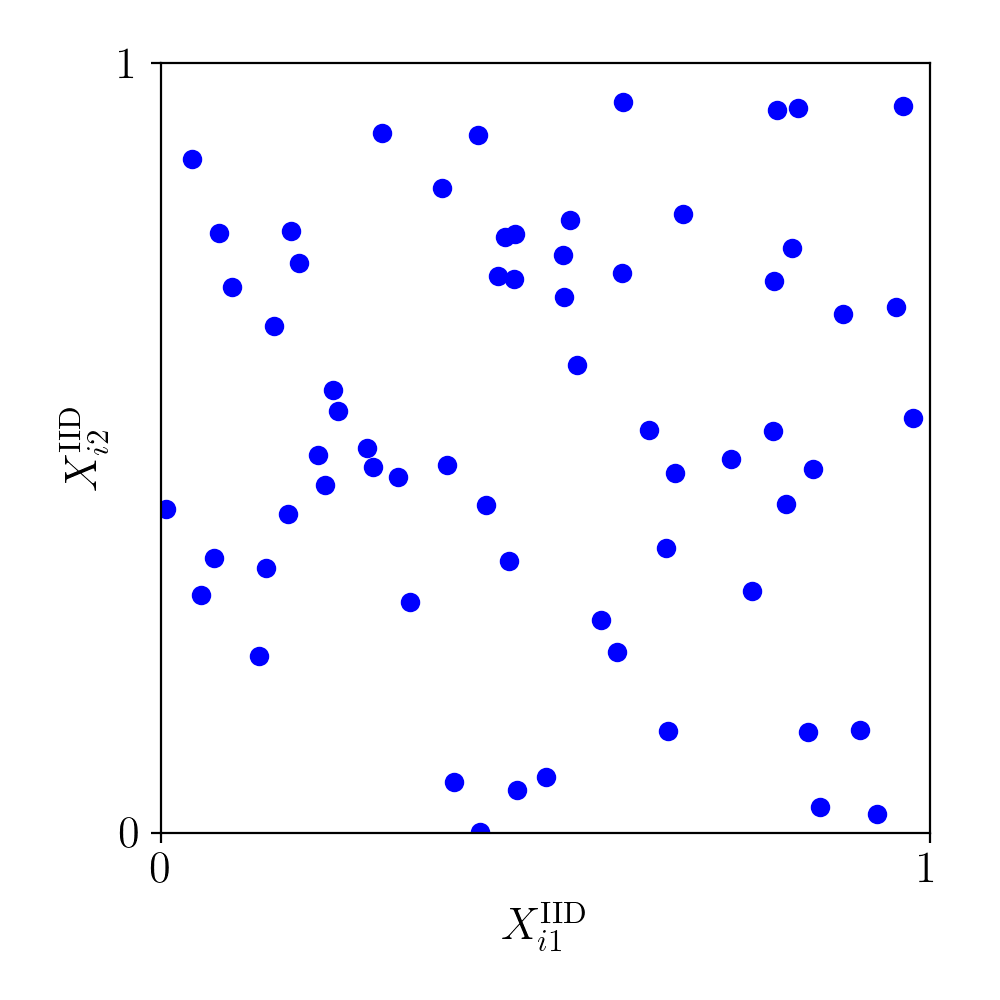
\includegraphics[height=5cm]{QMCSoftwareArticle/figs/dd_iid_uniform_pts.png}
	\qquad
	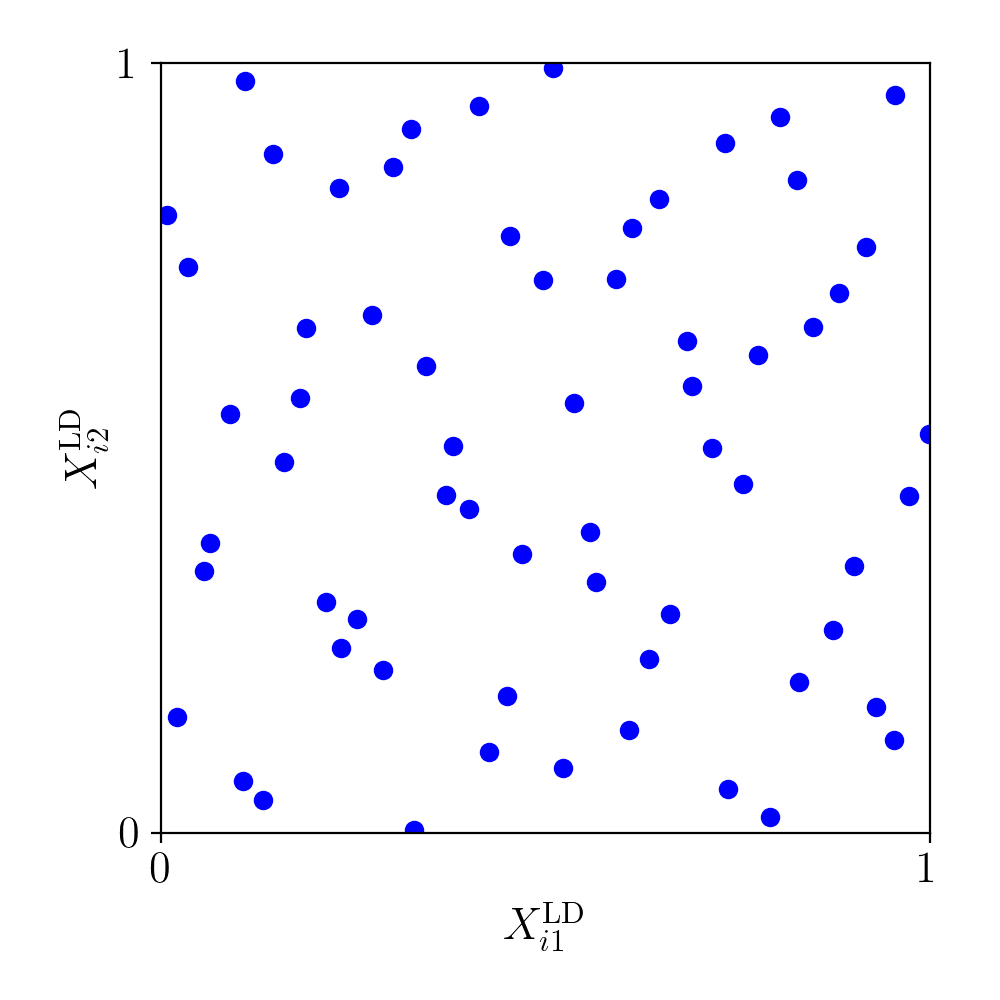
\includegraphics[height=5cm]{QMCSoftwareArticle/figs/dd_sobol_pts.png}
	\caption{IID points contrasted with LD points.  The LD points cover the square more evenly.}
	\label{fig:comparePts}
\end{figure}

LD sequences may be deterministic or random, but each point is carefully coordinated with the other so that they fill the domain well.  When we say that $\bsX_0, \bsX_1, \ldots \LDsim F$, we mean that for any positive integer $n$,  the \emph{empirical distribution} of $\bsX_0, \ldots, \bsX_{n-1}$, denoted $F_{\{\bsX_i\}_{i=0}^{n-1}}$,  approximates the target distribution, $F$, well (relative to $n$).  (The empirical distribution of a set assigns equal probability to each point.)  The measure of the difference between the empirical distribution of a set of points and the target distribution is called a \emph{discrepancy} and is denoted $D(\{\bsX_i\}_{i=0}^{n-1}, F)$.  This is the origin of the term ``low discrepancy'' points or sequences.  LD points by definition have a smaller discrepancy than IID points.  Figure \ref{fig:comparePts} contrasts IID uniform points with LD points, $\bsX^{\LD}_0, \bsX^{\LD}_1 \ldots \LDsim \calU[0,1]^2$, in this case linearly scrambled Sobol' points. For nearly all LD sequences, the target distribution is $\calU[0,1]^d$.

The error in using the sample mean to approximate the integral can be bounded according to the Koksma-Hlawka inequality and its extensions as the product of the discrepancy of the sampling sequence and the variation of the integrand, denoted $V(\cdot)$:
\begin{equation}
	\QMCPYabs{\mu - \hmu} = \QMCPYabs{\int_{\calX} f(\bsx) \, \D (F - F_{\{\bsX_i\}_{i=0}^{n-1}}) (\bsx)} \le D(\{\bsX_i\}_{i=0}^{n-1}, F) V(f),
\end{equation}
The variation is a (semi-) norm of the integrand in a suitable Banach space.  The discrepancy corresponds to the norm of the error functional for that Banach space.  For typical Banach spaces, the discrepancy of LD points is $\calO(n^{-1+\epsilon})$, which is a higher convergence order than for IID points.  For details, the reader is referred to the references.  For our purposes, we expect the reader to see in Figure \ref{fig:comparePts} that the LD points cover the integration domain more evenly than IID points.  In the examples below the reader will see the demonstrably smaller cubature errors arising from using LD points.

In the sections that follow we first overview available QMC software.  We next describe an architecture for good QMC software, i.e., what are the key components and how should they interact.  We then describe how we have implemented this architecture in QMCPy.  Finally, we summarize further directions that we hope QMCPy and related software projects will take.  Those interested in following the development of QMCPy or even contributing to that development are urged to visit the GitHub repository at \href{https://qmcsoftware.github.io/QMCSoftware/}{\nolinkurl{https://qmcsoftware.github.io/QMCSoftware/}}.

\section{Available Software for QMC} \label{CDHJS_sec:available}
QMC software spans  LD sequence generators, algorithms, and applications.  We review the better known software collections, recognizing that some software overlaps multiple categories.
Software focusing on generating high quality LD sequences  or their generators includes
\begin{description}[format=\textup,format=\textbf]
% https://tex.stackexchange.com/questions/74279/how-to-add-bullets-to-description-lists
	\item[BRODA] Sobol' sequences in C, MATLAB, and Excel \cite{BRODA20a},
	\item[Burkhardt] various QMC software in C++, Fortran, MATLAB, \& Python \cite{Bur20a},
	\item[LatNet Builder] Generating vectors/matrices for lattices and digital nets \cite{LEcEtal22a,LatNet},
	\item[MATLAB] Sobol' and Halton sequences, commercial \cite{MAT9.9},
	\item[MPS] Magic Point Shop, lattices and Sobol' sequences \cite{Nuy17a},
	\item[Owen] Randomized Halton sequences in R \cite{Owe20a},
	\item[PyTorch] Scrambled Sobol' sequences \cite{PyTorch},
	\item[QMC.jl] LD Sequences in Julia \cite{Rob20a}, and
	\item [qrng]  Sobol', Halton, and Korobov sequences in R \cite{QRNG2020}.
\end{description}
Software focusing on QMC algorithms and applications includes
\begin{description}[format=\textup,format=\textbf]
	\item[GAIL] Automatic (Q)MC stopping criteria in MATLAB \cite{ChoEtal20a},
	\item[ML(Q)MC] Multi-Level (Quasi-)Monte Carlo routines in C++, MATLAB, Python, and R \cite{GilesSoft},
	\item[OpenTURNS] Open source initiative for the Treatment of Uncertainties, Risks 'N Statistics in Python \cite{OpenTURNS},
	\item[QMC4PDE] QMC for elliptic PDEs with random diffusion coefficients \cite{KuoNuy16a},
	\item[SSJ] Stochastic Simulation in Java \cite{SSJ}, and
	\item[UQLab] Framework for Uncertainty Quantification in MATLAB \cite{UQLab2014}.
\end{description}

The sections that follow describe QMCPy \cite{QMCPy2020a}, which is our attempt to combine the best of the above software under a common user interface written in Python 3.  The choice of language was determined by the desire to make QMC software accessible to a broad audience, especially the tech industry.

\section{Components of QMC Software}
QMC cubature can be summarized as follows.  We want to approximate the integral oe expectation, $\mu$, well by the sample mean, $\hmu$, where \eqref{eq:integral}, \eqref{eq:fintegral}, and \eqref{eq:samplemean} combine to give
\begin{multline} \label{eq:cubSummary}
	\mu : = \int_\calT g(\bst) \, \lambda(\bst) \, \D \bst  = \bbE[f(\bsX)] = \int_\calX f(\bsx) \, \varrho(\bsx) \, \D \bsx \approx \frac 1n \sum_{i=0}^{n-1} f(\bsX_i) =: \hmu, \\
	 \bsX_0, \bsX_1, \ldots \sim F.
\end{multline}
This requires four components, which we implement as QMCPy classes.

\begin{description}[format=\textup,format=\textbf]

	\item[Discrete Distribution] that produces $\bsX_0, \bsX_1, \dots$ mimicking the distribution $F$, which typically is $\calU[0,1]^d$;

	\item[True Measure] $\bst \mapsto \lambda (\bst) \D \bst$ that defines the original integral, e.g., Gaussian or Lebesgue;

	\item[Integrand] $g$ that  defines the original integral, plus the transformed version, $f$, to fit the discrete distribution; and

	\item[Stopping Criterion] that determines how large $n$ should be to ensure that $\QMCPYabs{\mu - \hmu_n} \le \varepsilon$.
\end{description}

The software libraries referenced in Section \ref{CDHJS_sec:available} provide one or more of these components. QMCPy combines multiple examples of them all under and object oriented framework. Each example is implemented as a concrete class that realizes the properties and methods required by the abstract class for that component. The following sections detail descriptions and use cases for each component and select implementations.

Thorough documentation of all QMCPy classes can be found in \cite{QMCPyDocs}. Demonstrations of how QMCPy work are given in Google Colab notebooks \cite{QMCPyTutColab2020,QMCPyTutColab2020_paper} \AGSComment{Update \cite{QMCPyTutColab2020_paper}'s link}. The project may be installed from PyPI into your Python 3 environment via the command \texttt{pip install qmcpy}. In the codes that follows, we assume QMCPy has been imported alongside Numpy \cite{numpy}
%and Scipy \cite{scipy}
via
\lstinputlisting[style=Python]{QMCSoftwareArticle/python/import.txt}

\section{Discrete Distributions}

LD sequences typically mimic $\calU[0,1]^d$, which we assume here.  Good sequences for other distributions are obtained by transformations in the next section.

QMCPy implements \emph{extensible} LD sequences, i.e., those that allow practitioners to obtain and use $\bsX_n, \bsX_{n+1}, \ldots $ without discarding the existing $\bsX_0, \ldots, \bsX_{n-1}$.  Halton sequences do not have preferred sample sizes $n$, but integration lattices and digital sequences do.  These latter two also have an elegant group structure, which we summarize in Table \ref{tab:GroupProp}.  For simplicity we restrict ourselves to the case where the first $n = 2^m$ points of these LD sequences form a group under the addition operator $\oplus$.

\begin{table}
	\centering
	\caption{Properties of lattices and digital net sequences.  Note that they share group properties but also have distinctives.} \label{tab:GroupProp}
\[
	\renewcommand{\arraystretch}{1.3}
\begin{array}{c@{\qquad}c}
	\toprule
	\multicolumn{2}{c}{\text{Define \ldots}} \\
	\multicolumn{2}{c}{\bsZ_1, \bsZ_2, \bsZ_4, \ldots \in [0,1)^d \text{ chosen well} } \\
	\multicolumn{2}{c}{
	\bsZ_{i} := i_0  \bsZ_1 \oplus i_1 \bsZ_{2} \oplus + i_2  \bsZ_{4} \oplus  i_3  \bsZ_{8} + \cdots
	\quad
	\text{for }i = i_0 +i_1 2 + i_2 4 + i_3 8 + \cdots, \; i_\ell \in \{0,1\}} \\
    \multicolumn{2}{c}{\bsX_i := \bsZ_i \oplus \bsDelta, \qquad \text{where }\bsDelta \IIDsim [0,1)^d} \\  \hline
	\text{Rank-1 Integration Lattices} & \text{Digital Nets} \\
		\bst \oplus \bsx : = (\bst + \bsx) \bmod \bsone & \bst \oplus \bsx := \text{binary digitwise addition} \\
		 \text{require } \begin{array}{l} \bsZ_1 = (1/2, \ldots, 1/2) \\
		 	\bsZ_{2^{m}} \oplus \bsZ_{2^{m}} = \bsZ_{2^{m-1}} \quad \forall m \in \bbN \end{array}
		\\
\toprule
\multicolumn{2}{c}{\text{Then it follows that \ldots}} \\
	\multicolumn{2}{c}{\left . \begin{array}{r}
			\calP_m := \{\bsZ_0, \ldots, \bsZ_{2^m-1}\}, \quad
			\bsZ_i \oplus \bsZ_j \in \calP_m \\
			\calP_{\bsDelta,m} := \{\bsX_0, \ldots, \bsX_{2^m-1}\}, \quad
			\bsX_i \oplus \bsX_j \ominus \bsX_k \in \calP_{\bsDelta,m}
	\end{array} \right \}\quad \begin{array}{l}\forall  i,j,k \in \{0, \ldots, 2^{m} -1\} \\ \forall m \in \bbN_0\end{array}} \\
\bottomrule
\end{array}
\]
\end{table}

We illustrate lattice and Sobol' sequences using QMCPy. First, we create an instance of a $d=2$ dimensional \texttt{Lattice} object of the  \texttt{DiscreteDistribution} abstract class. Then we generate the first eight (non-randomized) points in this lattice.
\lstinputlisting[style=Python]{QMCSoftwareArticle/python/dd_lattice.txt}
The first three generators for this lattice are $\bsZ_1 = (0.5, 0.5)$, $\bsZ_2 = (0.25, 0.75)$, and $\bsZ_4 = (0.125, 0.375)$.  One can check that $(\bsZ_2 + \bsZ_4) \bmod \bsone = (0.375, 0.125) = \bsZ_6$, as Table \ref{tab:GroupProp} specifies.

The randomized shift has been turned off above to illuminate the group structure.  In practice, we normally include the randomization to ensure that there are no points on the boundary of $[0,1]^d$.  Then, when points are transformed to mimic distributions such as the Gaussian, no LD points will be transformed to infinity.  Turning off the randomization generates a warning.

Now, we generate Sobol' points using a similar process as we did for lattice points.  Sobol' sequences are one of the most popular example of digital sequences.
\lstinputlisting[style=Python]{QMCSoftwareArticle/python/dd_sobol.txt}
Here, $\bsZ_4$ differs from that for lattices, but more importantly, addition for digital sequences differs from that for lattices.  Using digitwise addition for digital sequences, we can confirm that according to Table \ref{tab:GroupProp},
\begin{multline*}
\bsZ_2 \oplus_{\dig} \bsZ_4 = (0.25,0.75)  \oplus_{\dig} (0.125,0.625) \\
=  ({}_20.010,{}_20.110)  \oplus_{\dig} ({}_20.001,{}_20.101) = ({}_20.011,{}_20.011) \\
= (0.375,0.375) = \bsZ_6.
\end{multline*}

By contrast, if we construct a digital sequence using the generators for the lattice above with $\bsZ_2 = (0.25, 0.75)$, and $\bsZ_4 = (0.125, 0.875)$, we would obtain
\begin{multline*}
\bsZ_6 = \bsZ_2 \oplus_{\dig} \bsZ_4   = ({}_20.010,{}_20.110)  \oplus_{\dig} ({}_20.001,{}_20.111)  \\
= ({}_20.011,{}_20.001) = (0.375, 0.125),
\end{multline*}
which differs from the $\bsZ_6=(0.375, 0.625)$ constructed for lattices.  To emphasize, lattices and digital sequences are different, even if they share the same generators, $\bsZ_1, \bsZ_2, \bsZ_4, \ldots$.

The examples of \texttt{qp.Lattice} and \texttt{qp.Sobol} illustrate how QMCPy LD generators share a common user interface.  The dimension is specified when the instance is constructed, and the number of points is specified when the \texttt{gen\_samples} method is called.  Following Python practice, parameters can be input without specifying their names if they are input in the prescribed order.  QMCPy also includes Halton sequences and IID sequences, again deferring details to the QMCPy documentation \cite{QMCPyDocs}.

A crucial difference between IID generators and LD generators is reflected in the behavior of generating $n$ points.  For an IID generator, asking for $n$ points repeatedly gives you different points each time because they are meant to be random and independent.
\lstinputlisting[style=Python]{QMCSoftwareArticle/python/dd_iidone.txt}
Your output may look different depending on the seed used to generate these random numbers.

On the other hand for an LD generator, asking for $n$ points repeatedly gives you \emph{the same} points each time because they are meant to be the first $n$ points of a given LD sequence.
\lstinputlisting[style=Python]{QMCSoftwareArticle/python/dd_latticeone.txt}
Here we allow the randomization so that the first point in the sequence is not the origin.  To obtain the \emph{next} $n$ points one may specify the start and ending indices of the sequence.
\lstinputlisting[style=Python]{QMCSoftwareArticle/python/dd_latticenextone.txt}

Figure \ref{fig:increase_n} shows how increasing the number of lattice and Sobol' LD points through powers of two fills in the gaps in an even way.

\begin{figure}
	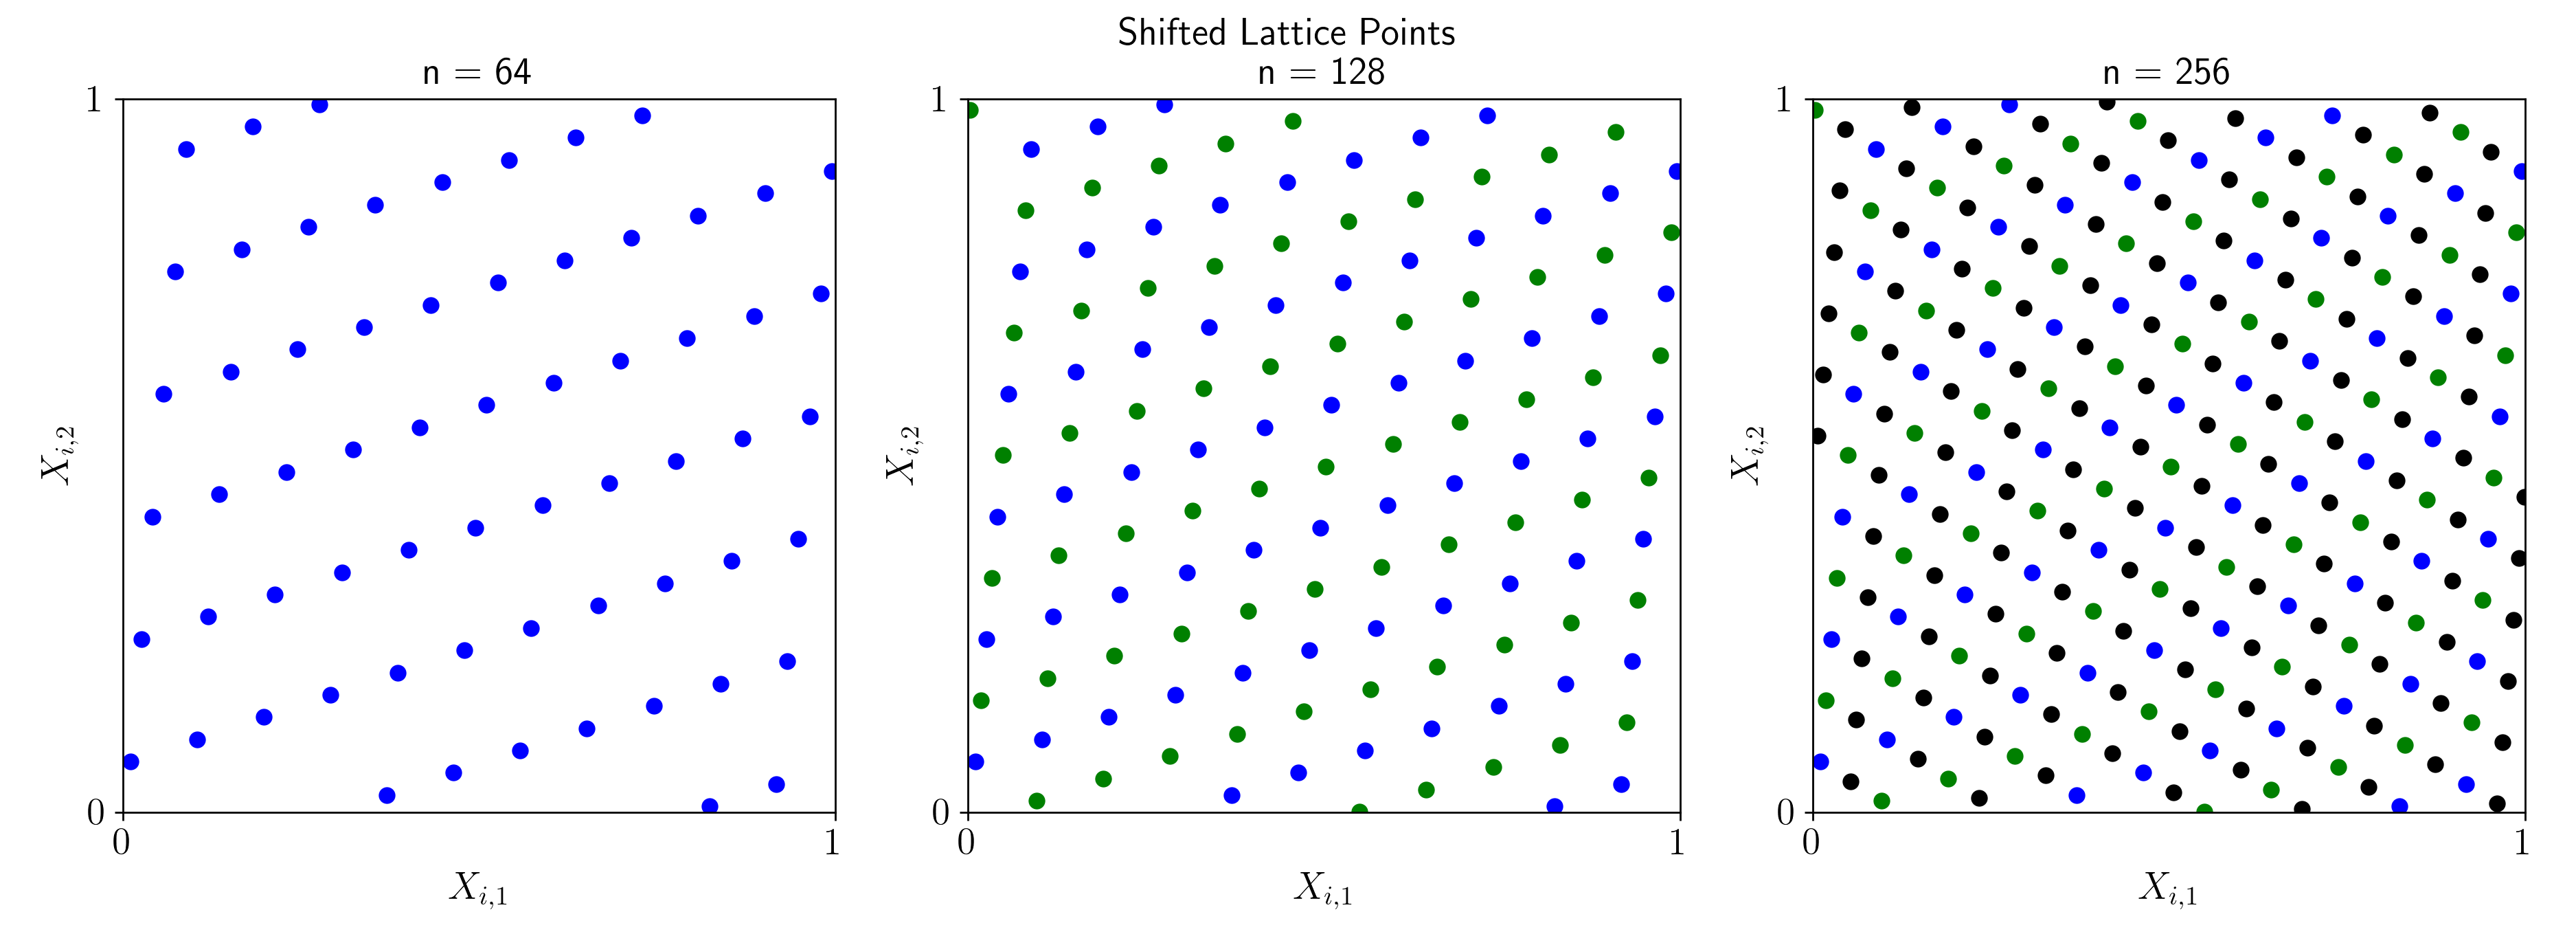
\includegraphics[width=1\textwidth]{QMCSoftwareArticle/figs/dd_lattice_successive.png}
	\qquad
	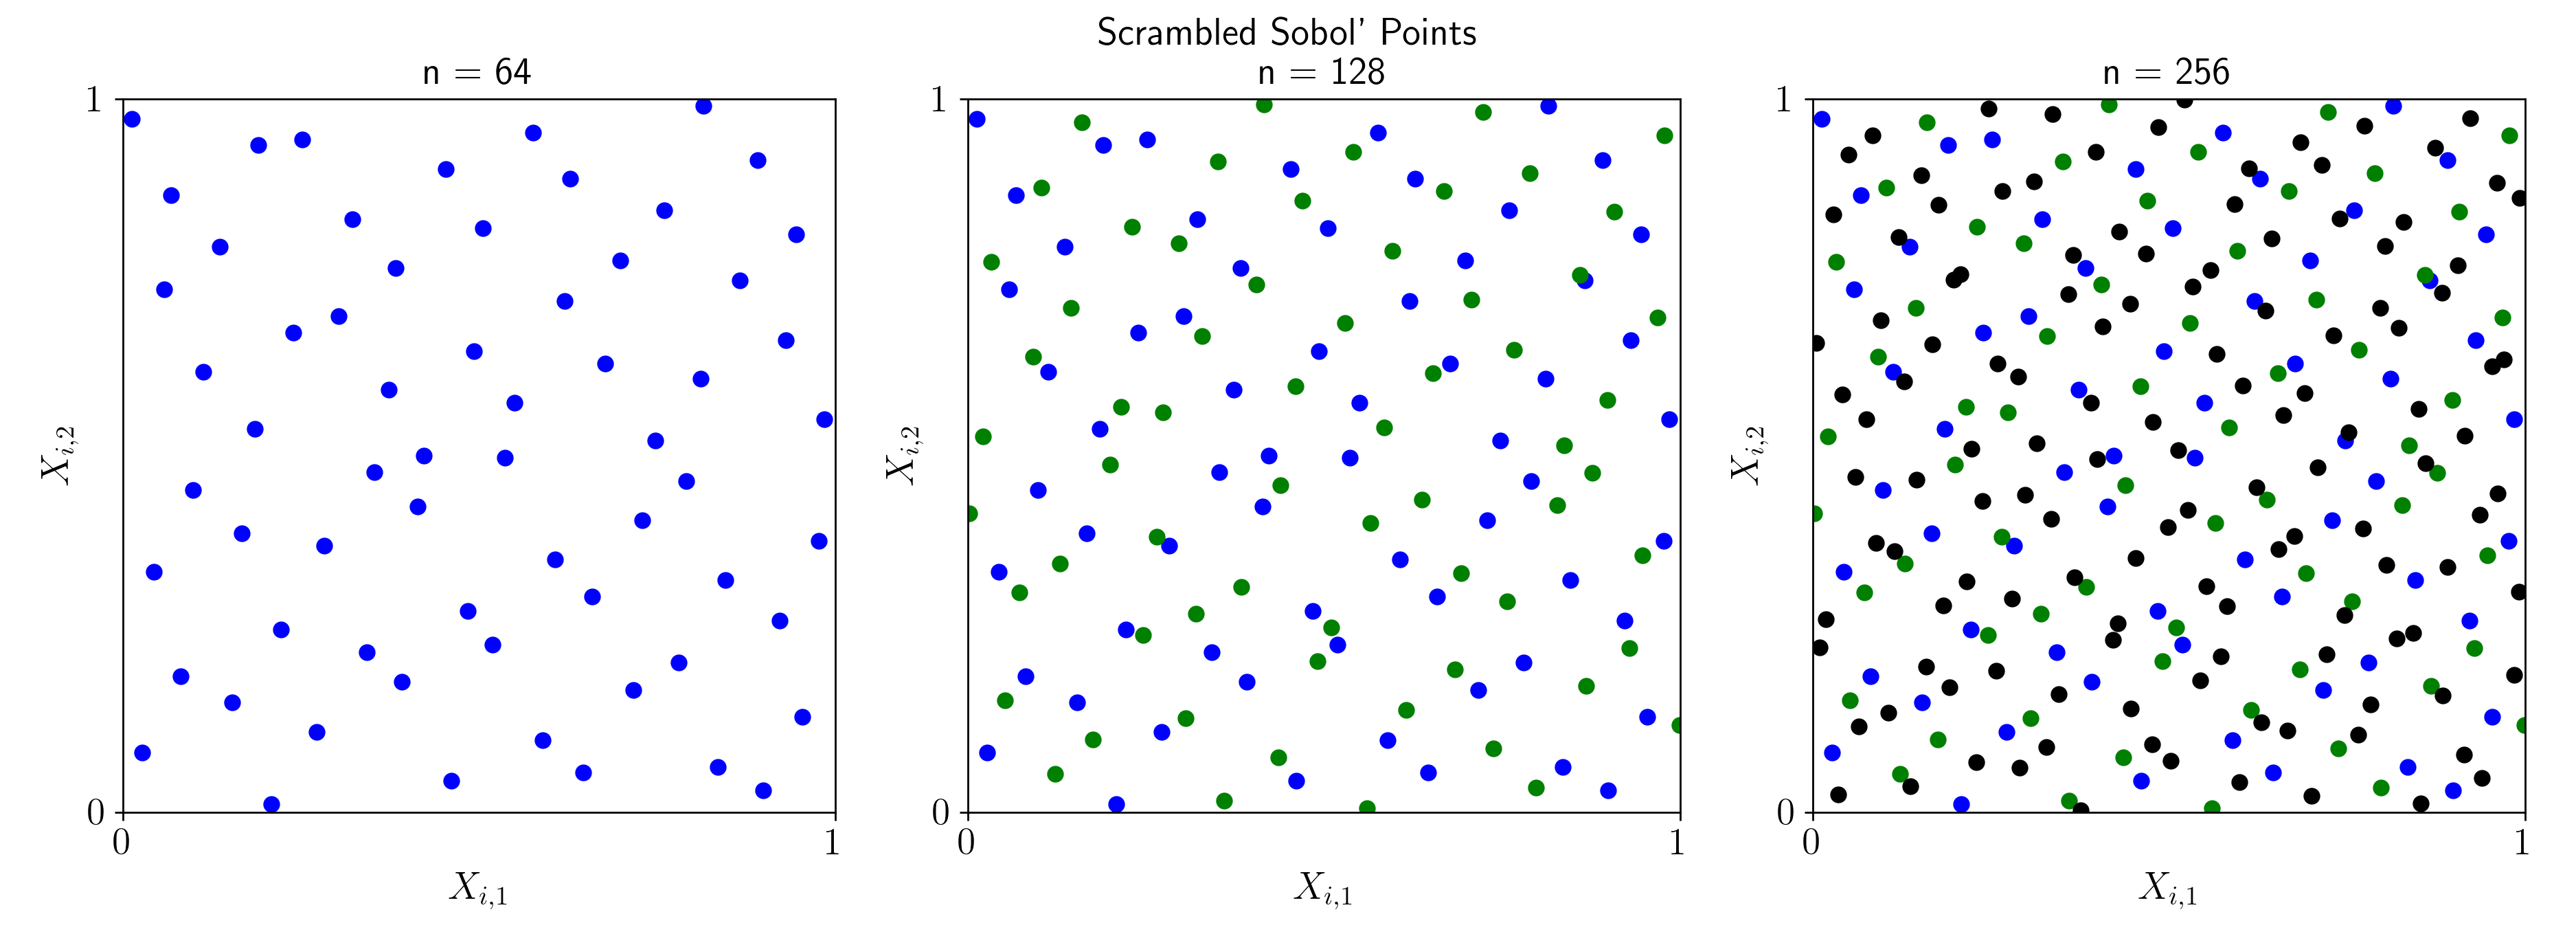
\includegraphics[width=1\textwidth]{QMCSoftwareArticle/figs/dd_sobol_successive.png}
	\caption{Randomized lattice and Sobol' points mimicking a $\calU[0,1]^2$ measure for $n = 64, 128,$ and 256. Note how increasing the number of points evenly fills in the gaps between points.}
	\label{fig:increase_n}
\end{figure}

\section{True Measures}

The LD sequences implemented as \text{DiscreteDistribution} objects typically mimic the $\calU[0,1]^d$ distribution.  However, we may need sequences to mimic other distributions.  This is implemented via variable transformations, $\bsPsi$.  In general, if $\bsX \sim \calU[0,1]^d$, then
\begin{subequations} \label{eq:exampleVarTrans}
\begin{gather}
\bsT = \bsPsi(\bsX) := \bsa  + (\bsb - \bsa) \odot \bsX \sim  \calU[\bsa,\bsb], \\
\label{eq:exampleVarTransGauss}
\bsT = \bsPsi(\bsX) := \bsa + \mA \bsPhi^{-1}(\bsX)  \sim \calN(\bsa, \mSigma), \\
\nonumber  \text{where }  \bsPhi^{-1}(\bsX) : = \begin{pmatrix} \Phi^{-1}(X_1) \\ \vdots \\ \Phi^{-1}(X_d)\end{pmatrix}, \qquad \mSigma = \mA \mA^T,
\end{gather}
\end{subequations}
and $\odot$ denotes term-by-term (Hadamard) multiplication.  Here, $\bsa$ and $\bsb$ are assumed to be finite, and $\Phi$ is the standard Gaussian distribution function.  Again we use ``$\sim$'' to denote mimicry, not necessarily in a probabilistic sense.

Figure \ref{fig:tm_ug} displays LD sequences transformed as described above to mimic a uniform and a Gaussian distribution.  The code to generate these points takes the following form of
\lstinputlisting[style=Python]{QMCSoftwareArticle/python/tm_uniform.txt}
for uniform points based on a Halton sequence, and
\lstinputlisting[style=Python]{QMCSoftwareArticle/python/tm_gaussian.txt}
for Gaussian points based on a lattice sequence.

\begin{figure}
	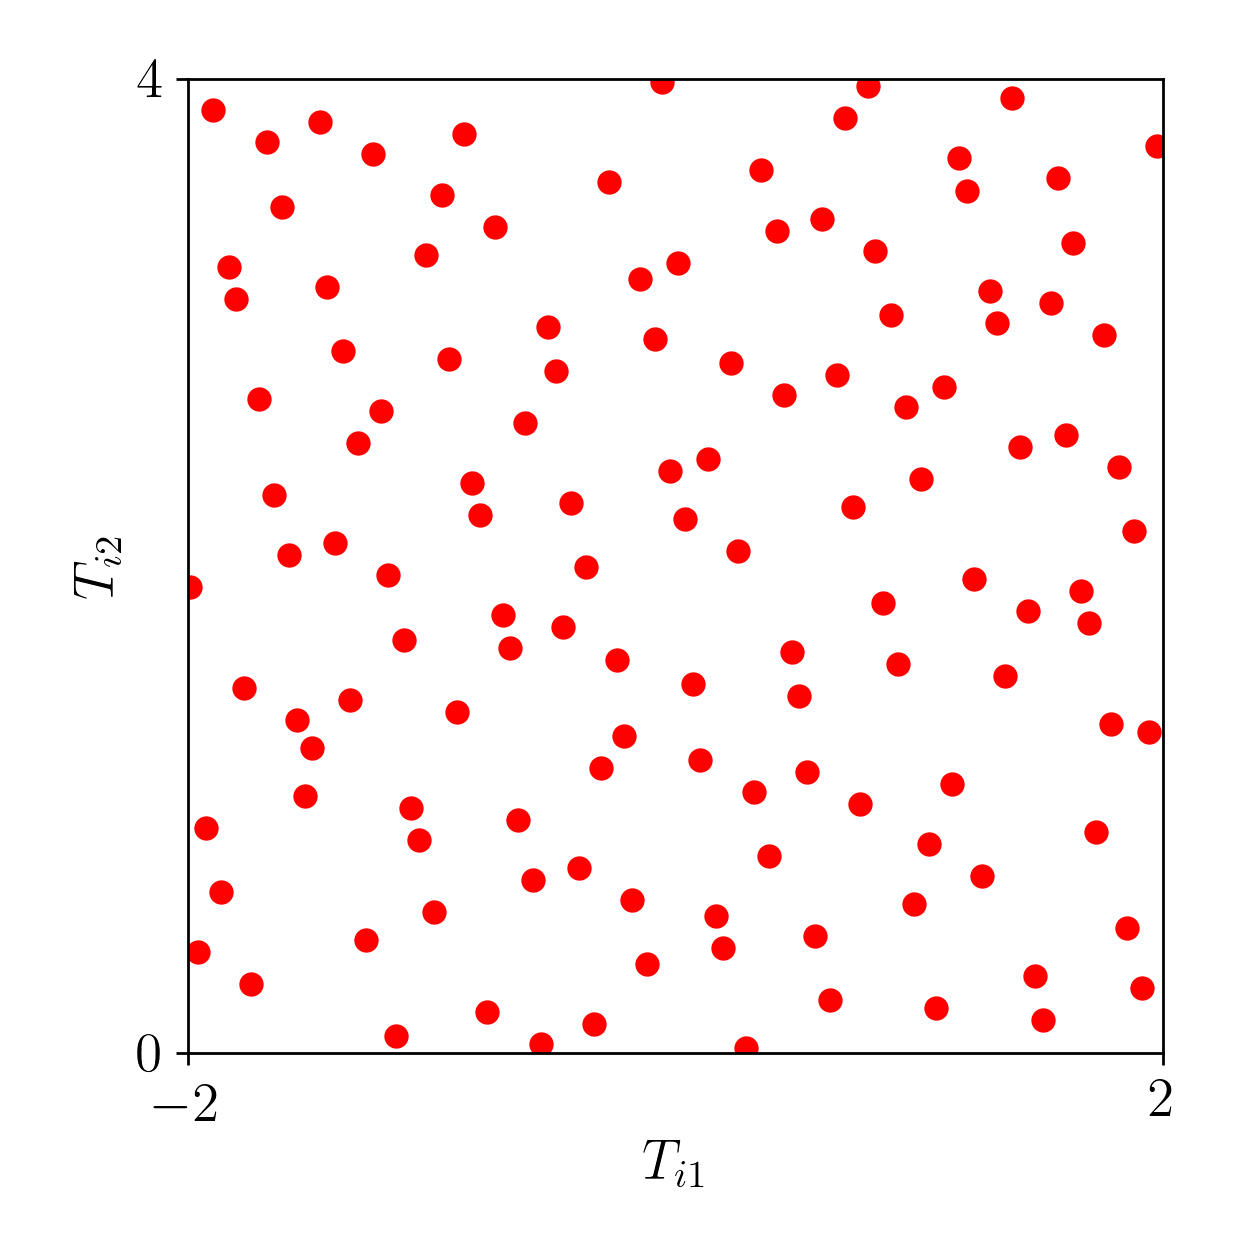
\includegraphics[width=.45\textwidth]{QMCSoftwareArticle/figs/tm_uniform.png}
	%	\quad
	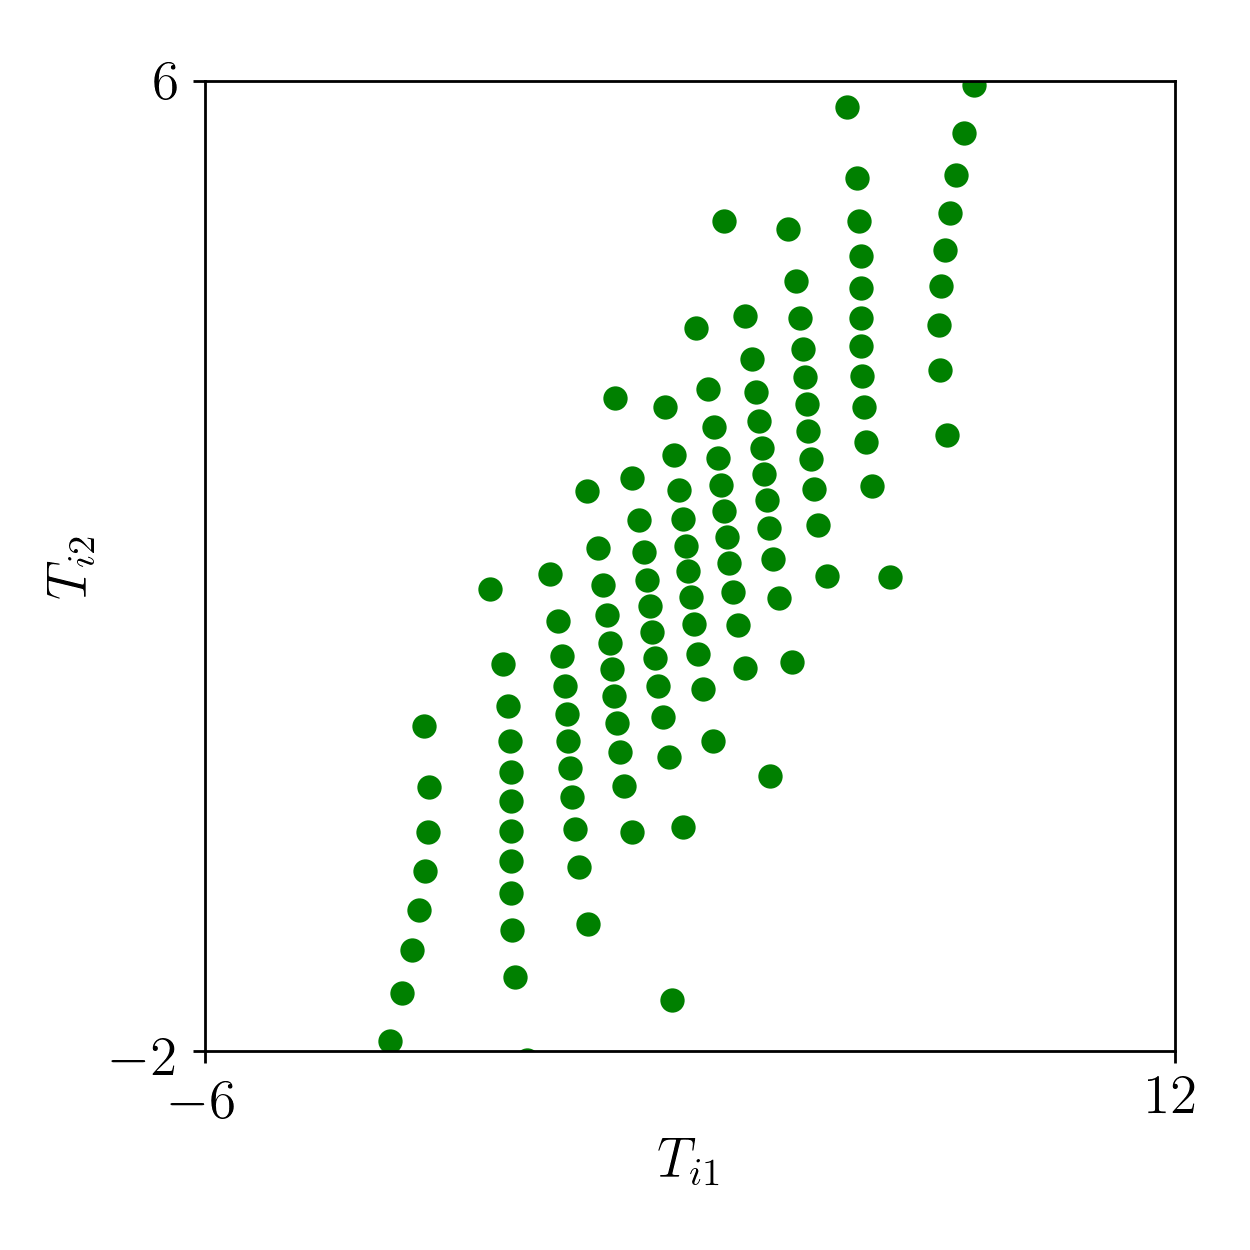
\includegraphics[width=.45\textwidth]{QMCSoftwareArticle/figs/tm_gaussian.png}
	\caption{Sobol' samples transformed to mimic a uniform $\calU\left(\begin{bmatrix} -2 \\ 0 \end{bmatrix}, \begin{bmatrix} 2 \\ 4 \end{bmatrix} \right)$ (left) and  Gaussian $\calN\left(\begin{bmatrix} 3 \\ 2 \end{bmatrix}, \begin{bmatrix} 9 & 5 \\ 5 & 4 \end{bmatrix} \right)$ (right).}
	\label{fig:tm_ug}
\end{figure}

The Brownian motion distribution arises often in financial risk applications.  Here the $d$ components of the variable $\bsT$ correspond to the Brownian motion at times $\tau/d, 2\tau/d, \ldots, \tau$, where $\tau$ is the time horizon.  The distribution is a special case of the Gaussian with covariance
\begin{equation} \label{eq:BMcov}
	\mSigma = (\tau/d) \bigl (\min(j,k) \bigr)_{j,k=1}^d
\end{equation}
and mean $\bsa$, which  correspond to a drift coefficient times $(\tau/d)(1, 2, \ldots, d)^T$. The code for generating a Brownian motion is
\lstinputlisting[style=Python]{QMCSoftwareArticle/python/tm_brownian_motion.txt}
Figure \ref{fig:tm_bm} displays a Brownian motion based on Sobol' sequence with and without a drift.

\begin{figure}
	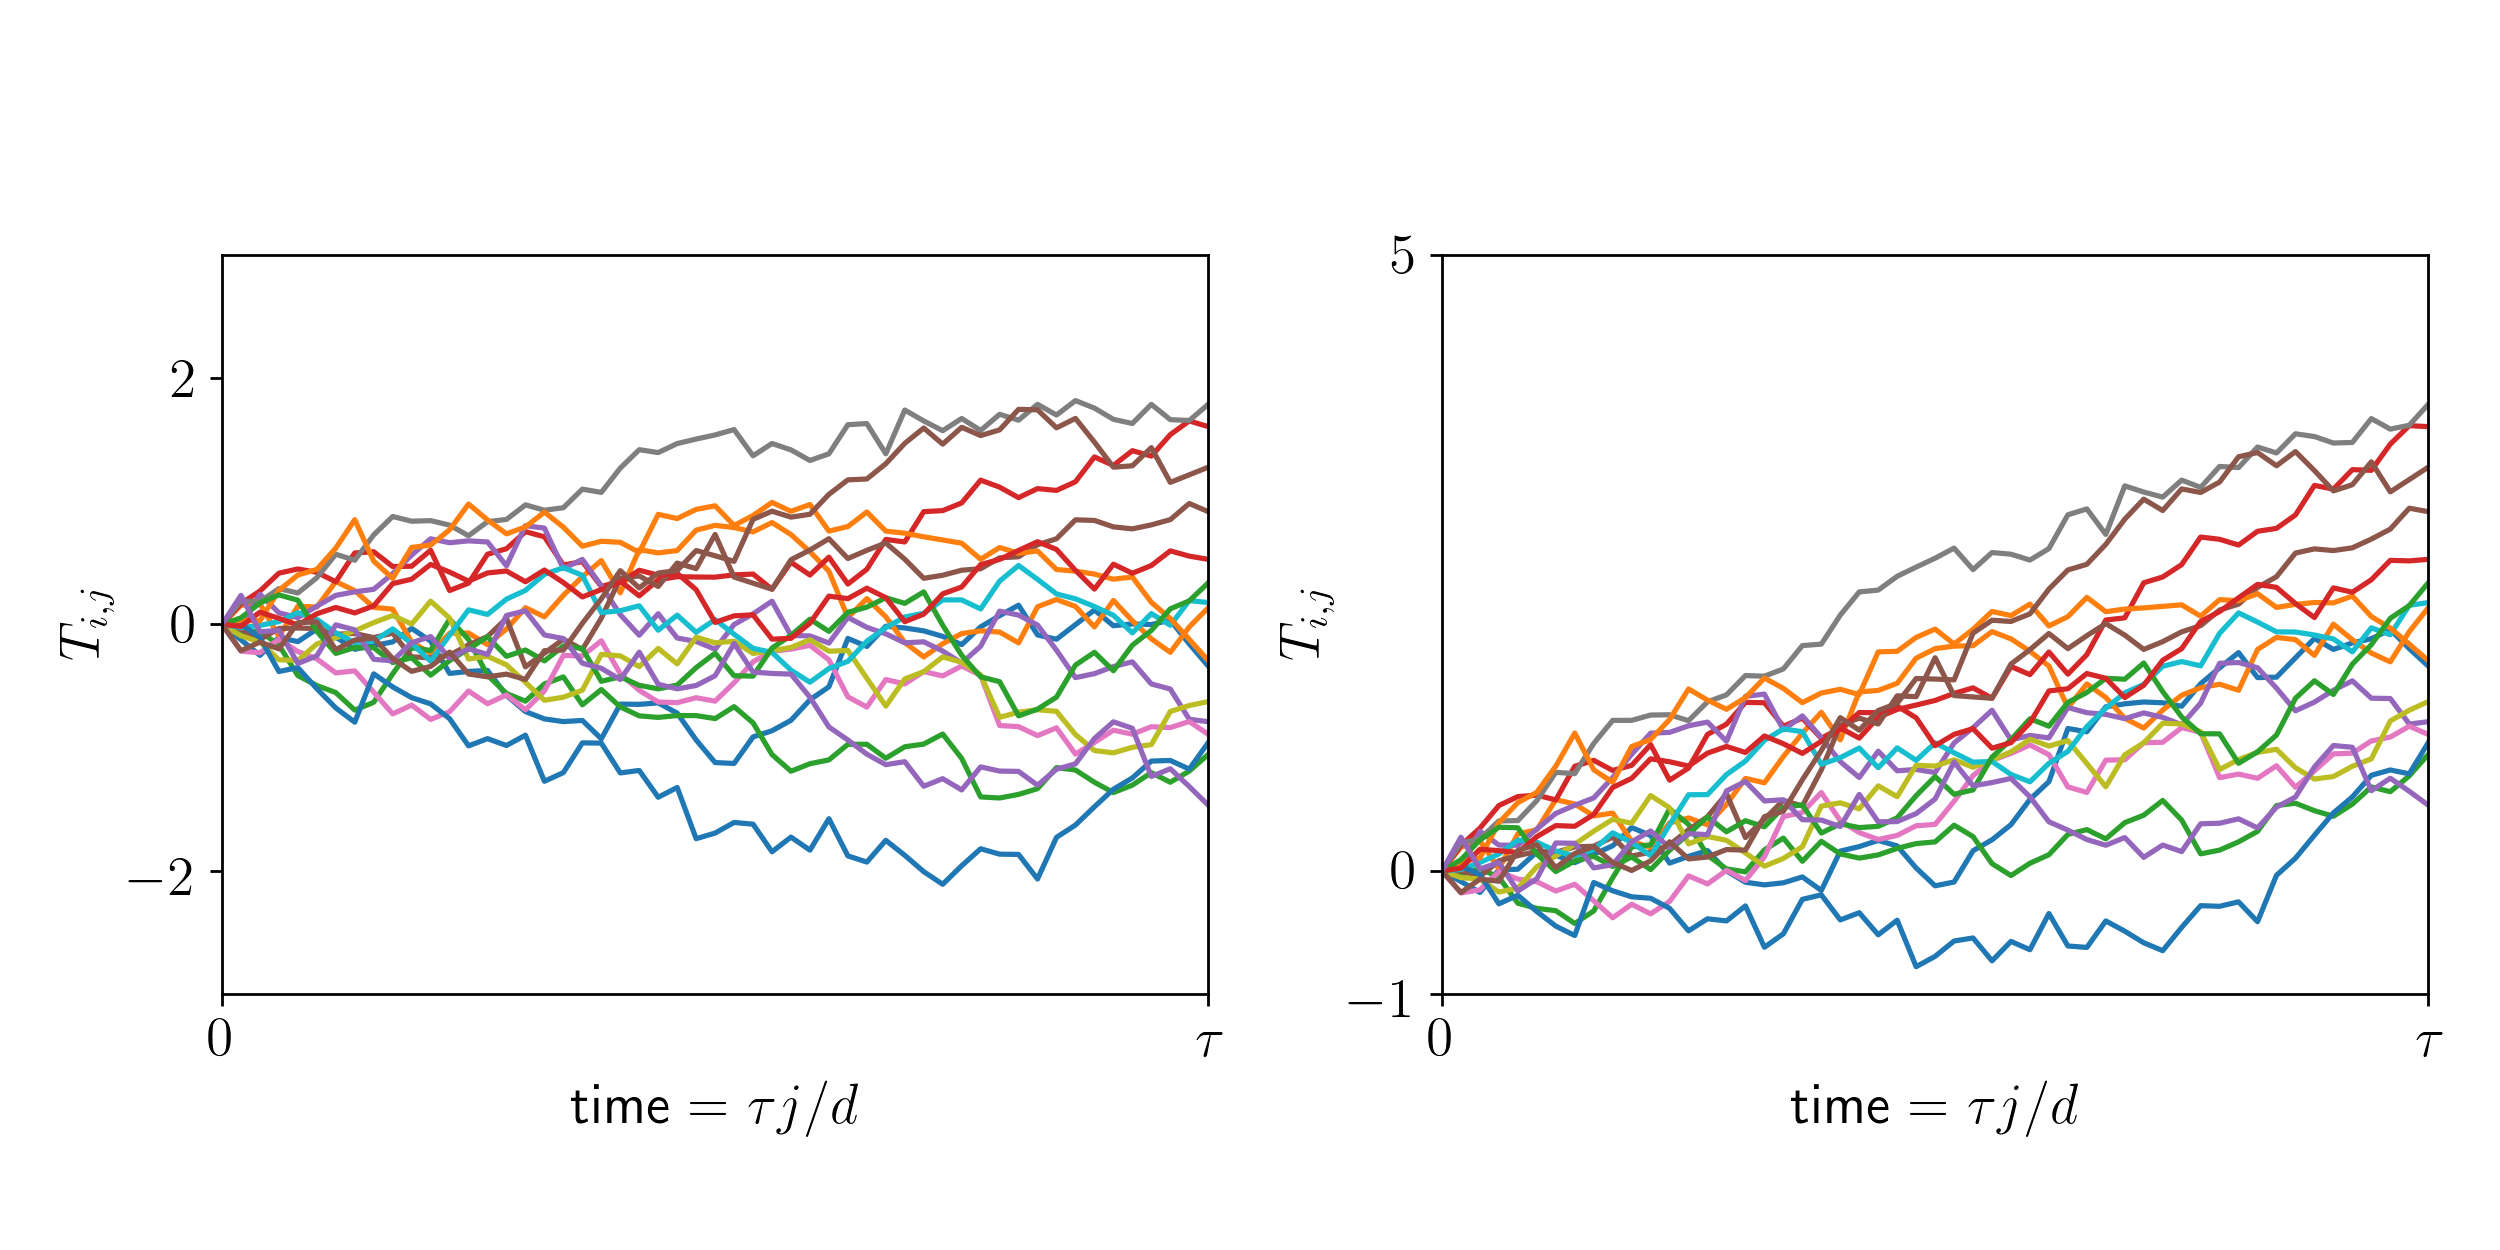
\includegraphics[width=1\textwidth]{QMCSoftwareArticle/figs/tm_bm.png}
	\caption{Sobol' samples transformed to mimic a 32-dimensional Brownian Motion without drift (left) and with drift coefficient 2 (right).}
	\label{fig:tm_bm}
\end{figure}

\section{Integrands}

Let's return now to the integration problem in \eqref{eq:integral}, which we must rewrite as \eqref{eq:fintegral}.  We choose a transformation of variables defined as $\bst = \bsPsi(\bsx)$ where $\bsPsi:\calX \to \calT$.  This leads to
\begin{align}
	\nonumber
 \mu &= \int_\calT g(\bst) \, \lambda(\bst) \, \D \bst  = \int_\calX g\bigl(\bsPsi(\bsx)\bigr) \, \lambda\bigl(\bsPsi(\bsx)\bigr) \,\QMCPYabs{\frac{\partial \bsPsi}{\partial \bsx}} \, \D \bsx =  \int_\calX f(\bsx) \, \varrho(\bsx) \, \D \bsx  \\
 \label{eq:transVar}
  & \qquad \qquad \text{where } f(\bsx)  = g\bigl(\bsPsi(\bsx)\bigr)  \, \frac{\lambda(\bsPsi(\bsx))}{\varrho(\bsx)} \,\QMCPYabs{\frac{\partial \bsPsi}{\partial \bsx}},
\end{align}
and $\QMCPYabs{\partial \bsPsi/\partial \bsx}$ represents the Jacobian of the variable transformation.  The abstract class \texttt{Integrand} provides $f$ based on the user's input of $g$ and the \texttt{TrueMeasure} instance, which defines $\lambda$ and the transformation $\bsPsi$. Different choices of $\bsPsi$ lead to different $f$, which may give different rates of convergence of the cubature, $\hmu$ to $\mu$.

We illustrate the use of the \texttt{Integrand} class via an example of Keister \cite{Kei96}:
\begin{equation} \label{eq:KeisterIntegral}
	\mu
	= \int_{\bbR^d} \cos(\lVert \bst \rVert) \exp(-\bst^T \bst) \, \D \bst \\
	= \int_{\bbR^d} \underbrace{\pi^{d/2} \cos(\lVert \bst \rVert)}_{g(\bst)}\, \underbrace{\pi^{-d/2} \exp(-\bst^T \bst) }_{\lambda(\bst)} \, \D \bst.
\end{equation}
We will use QMC methods to approximate this integral, which means that it will be transformed according to \eqref{eq:transVar} for the case where $\calX = [0,1]^d$ and $\varrho(\bsx) = 1$.  Since $\lambda$ is the density for $\calN(0,\mI/2)$, it is natural to choose $\bsPsi$ according to \eqref{eq:exampleVarTransGauss} with $\mA = \sqrt{1/2} \, \mI$, in which case $\lambda(\bsPsi(\bsx)) \QMCPYabs{\partial \bsPsi/\partial \bsx} / \varrho(\bsx) = 1$, and so
\[
\mu = \int_{[0,1]^d} \underbrace{\pi^{d/2} \cos(\lVert \bsPsi(\bsx) \rVert)}_{f(\bsx)} \, \D \bsx, \qquad
\bsPsi(\bsx) := \sqrt{1/2} \,\bsPhi^{-1}(\bsx).
\]

The code below sets up an \texttt{Integrand} instance using QMCPy's \texttt{CustomFun} wrapper to tie a user-defined function $g$ into the QMCPy framework.  Then we evaluate the sample mean of $n=1000$ $f$ values obtained by sampling at transformed Halton points.
\lstinputlisting[style=Python]{QMCSoftwareArticle/python/i_keister.txt}
We have no indication yet of how accurate our approximation is.  This aspect of QMCPy is described in the next section.  Figure \ref{fig:ikc} visualizes sampling on the original integrand, $g$, and sampling on the transformed integrand, $f$.

\begin{figure}
	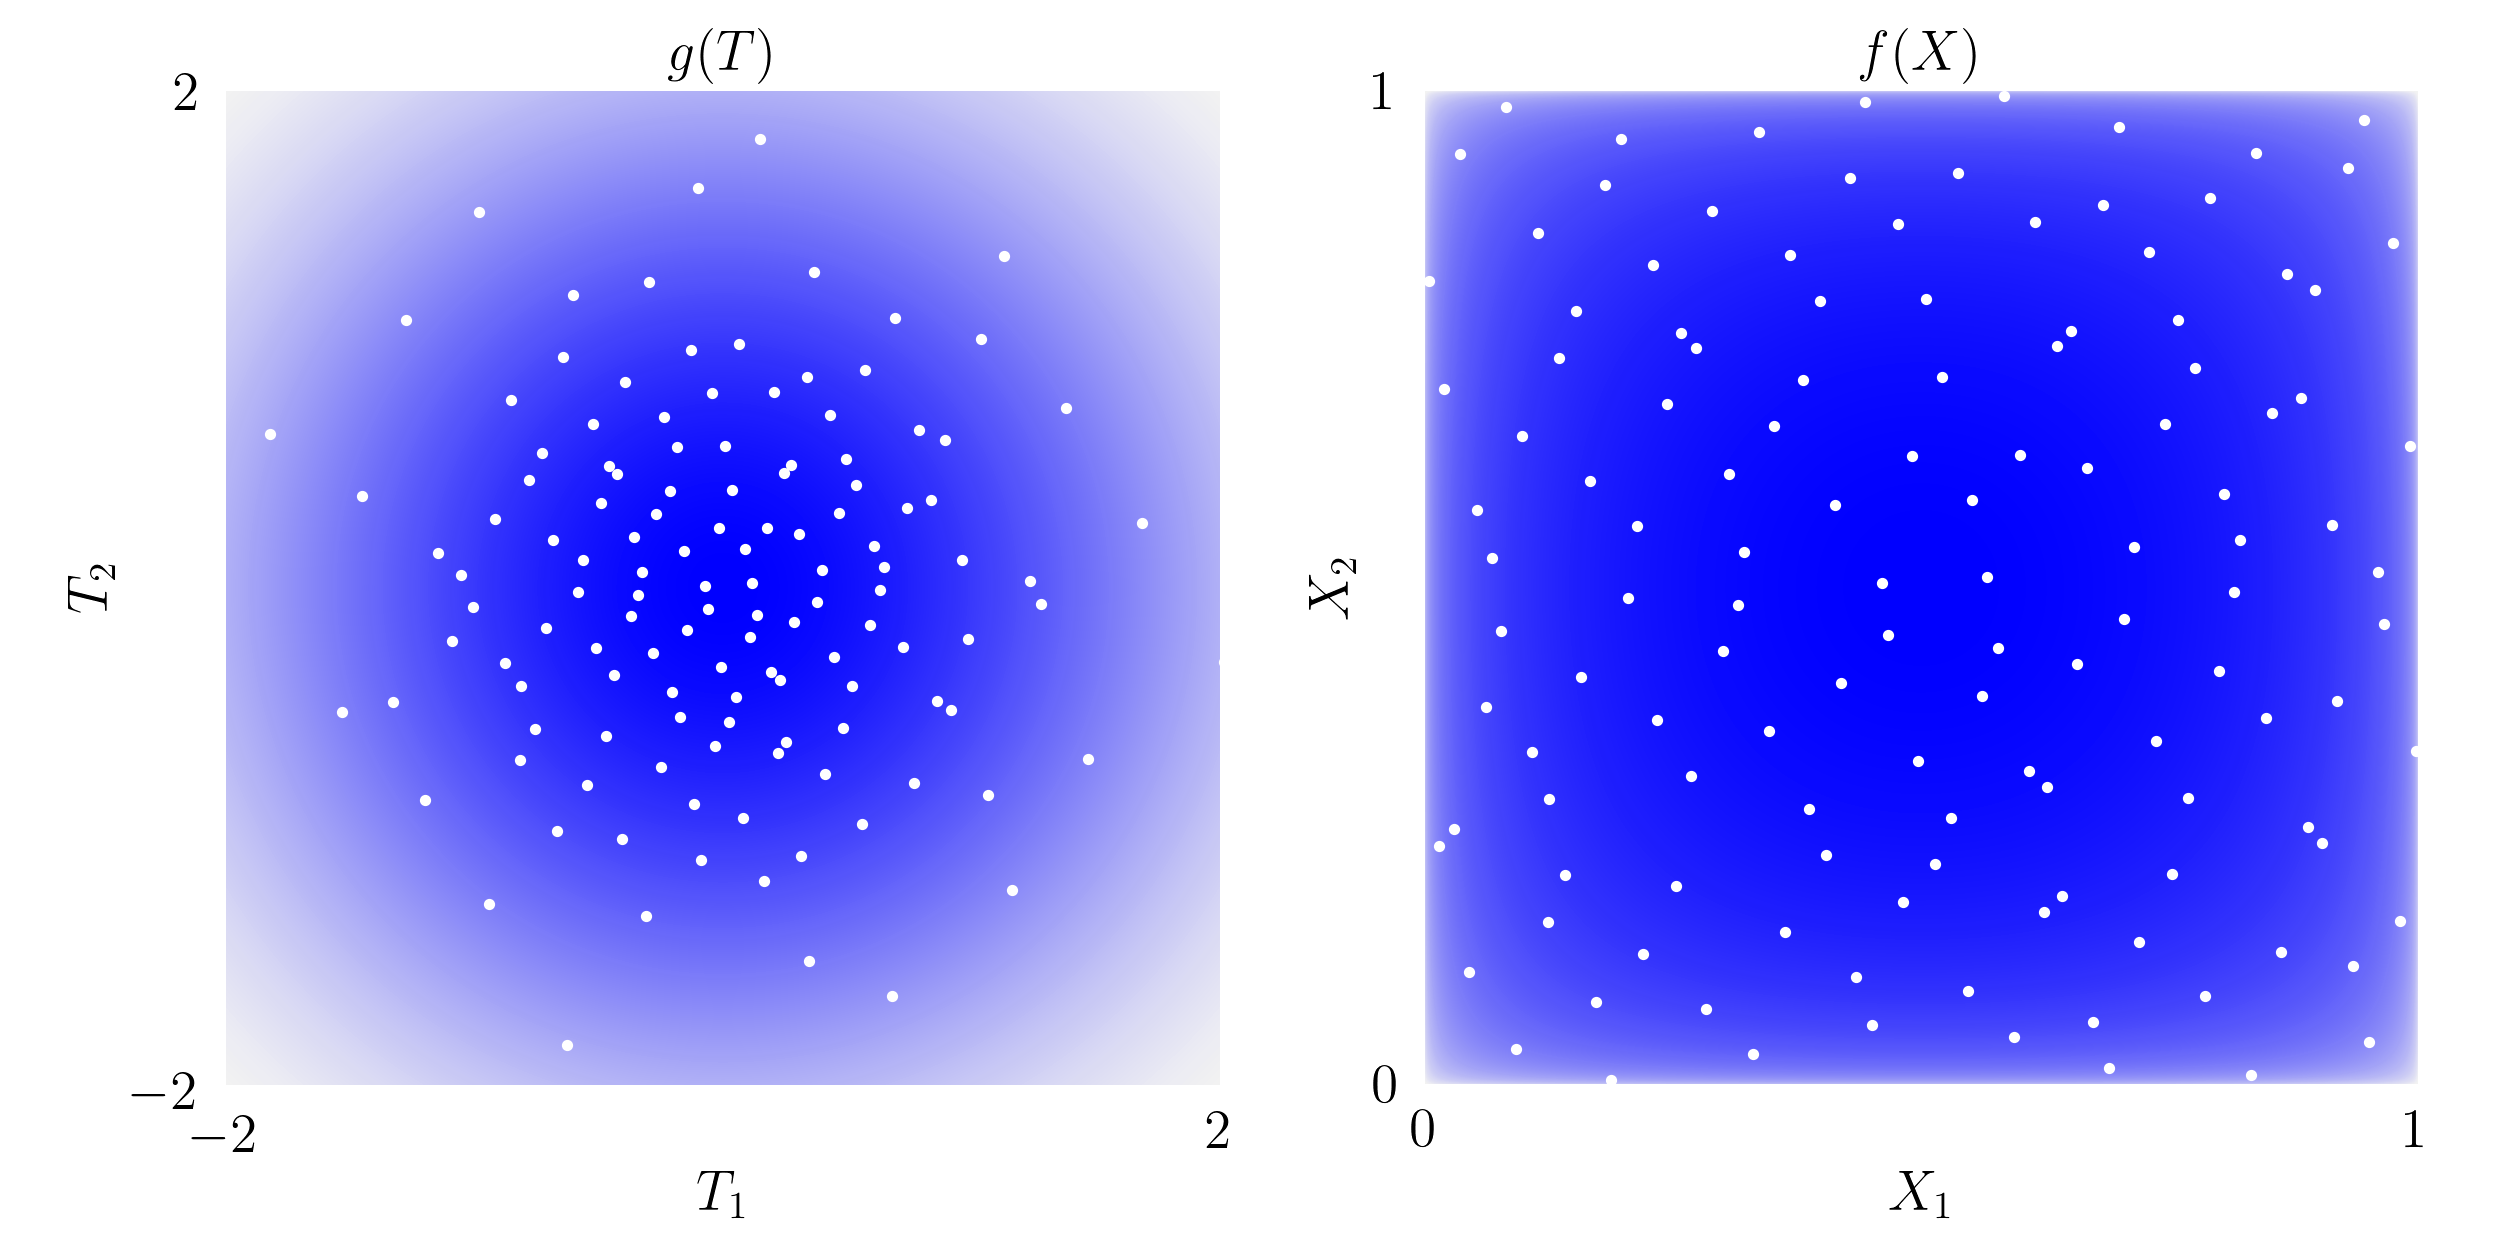
\includegraphics[height=6cm]{QMCSoftwareArticle/figs/i_keister_contours.png}
	\caption{Right: Sampling the transformed integrand $f$ at Halton points $\bsx \sim \calU[0,1]^2$. Left: Sampling the original integrand $g$ at $\bsPsi(\bsx)$ where $\bsPsi$ is defined in \eqref{eq:exampleVarTransGauss}.  } \label{fig:ikc}
\end{figure}

Another way to approximate the Keister integral in \eqref{eq:KeisterIntegral} is to write it as an integral with respect to the Lebesgue measure:
\begin{align*}
	\mu
	& = \int_{\bbR^d} \underbrace{\cos(\lVert \bst \rVert) \exp(-\bst^T \bst) }_{g(\bst)} \, \underbrace{1}_{\lambda(\bst)} \,\D \bst \\
	& = \int_{[0,1]^d} \underbrace{\cos(\lVert \bsPsi(\bsx) \rVert) \exp(-\bsPsi^T\!\!(\bsx) \bsPsi(\bsx)) \QMCPYabs{\frac{\partial \bsPsi}{\partial \bsx}} }_{f(\bsx)} \, \D \bsx,
\end{align*}
where $\bsPsi$ is any transformation from $\bbR^d$ to $[0,1]^d$.  QMCPy can perform the cubature this way as well.
\lstinputlisting[style=Python]{QMCSoftwareArticle/python/i_keisterLebesgue.txt}
The $\bsPsi$ chosen when transforming uniform points on the unit cube to fill the $\bbR^d$ is the one given by \eqref{eq:exampleVarTransGauss} with $\mA = \mI$.

In the examples above, one needed to input the correct $g$ into \texttt{CustomFun} along with the correct \texttt{TrueMeasure} $\lambda$ to define the integration problem. The \texttt{Keister} integrand included in the QMCPy library takes a more flexible approach of defining the integration problem $\mu$ in \eqref{eq:KeisterIntegral}. Selecting a different \texttt{sampler} $\bsPsi$ performs  \emph{importance sampling} which leaves $\mu$ unchanged.
\lstinputlisting[style=Python]{QMCSoftwareArticle/python/i_keisterBuiltIn.txt}

\section{Stopping Criteria} \label{CDHJS_sec:stopping_crit}

The \texttt{StoppingCriterion} object determines the number of samples $n$ that are required for the sample mean approximation $\hmu$ to be within error tolerance $\varepsilon$ of the true mean $\mu$.  Several QMC stopping criteria have been implemented in QMCPy, including replications, stopping criteria that track the decay of the Fourier complex exponential or Walsh coefficients of the integrand \cite{HicJim16a,HicEtal17a,JimHic16a}, and stopping criteria based on Bayesian credible intervals \cite{RatHic19a,JagHic22a}.

Let us return to the Keister example from the previous section.  After setting up  a default \texttt{Keister} instance via a Sobol' \texttt{DiscreteDistribution}, we choose a \texttt{StoppingCriterion} object that matches the \texttt{DiscreteDistribution}, inputting our desired tolerance.  Calling the  \texttt{integrate} method returns the approximate integral plus some useful information about the computation.
\lstinputlisting[style=Python]{QMCSoftwareArticle/python/sc_keister_qmc.txt}
The second output of the stopping criterion provides helpful diagnostic information.  This computation required $n=2^{13}$ Sobol' points and $0.028$ seconds to complete.  The error bound is $0.000517$, which falls below the absolute tolerance.

QMC, which uses LD sequences, is touted as providing substantially greater computational efficiency compared to IID MC.
Figure \ref{fig:sc_comp} compares the time and sample sizes needed to compute the $5$-dimensional Keister integral \eqref{eq:KeisterIntegral} using IID sequences and LD lattice sequences. Consistent with what is stated in Section \ref{CDHJS_sec:intro}, the error of IID MC is $\calO(n^{-1/2})$, which means that the time and sample size to obtain an absolute error tolerance of $\varepsilon$ is $\calO(\varepsilon^{-2})$.  By contrast, the  error of QMC using LD sequences is $\calO(n^{-1+\epsilon})$, which implies $\calO(\varepsilon^{-1-\epsilon})$ times and sample sizes.  We see that QMC methods often require orders of magnitude fewer samples that MC methods to achieve the same error tolerance.

\begin{figure}
	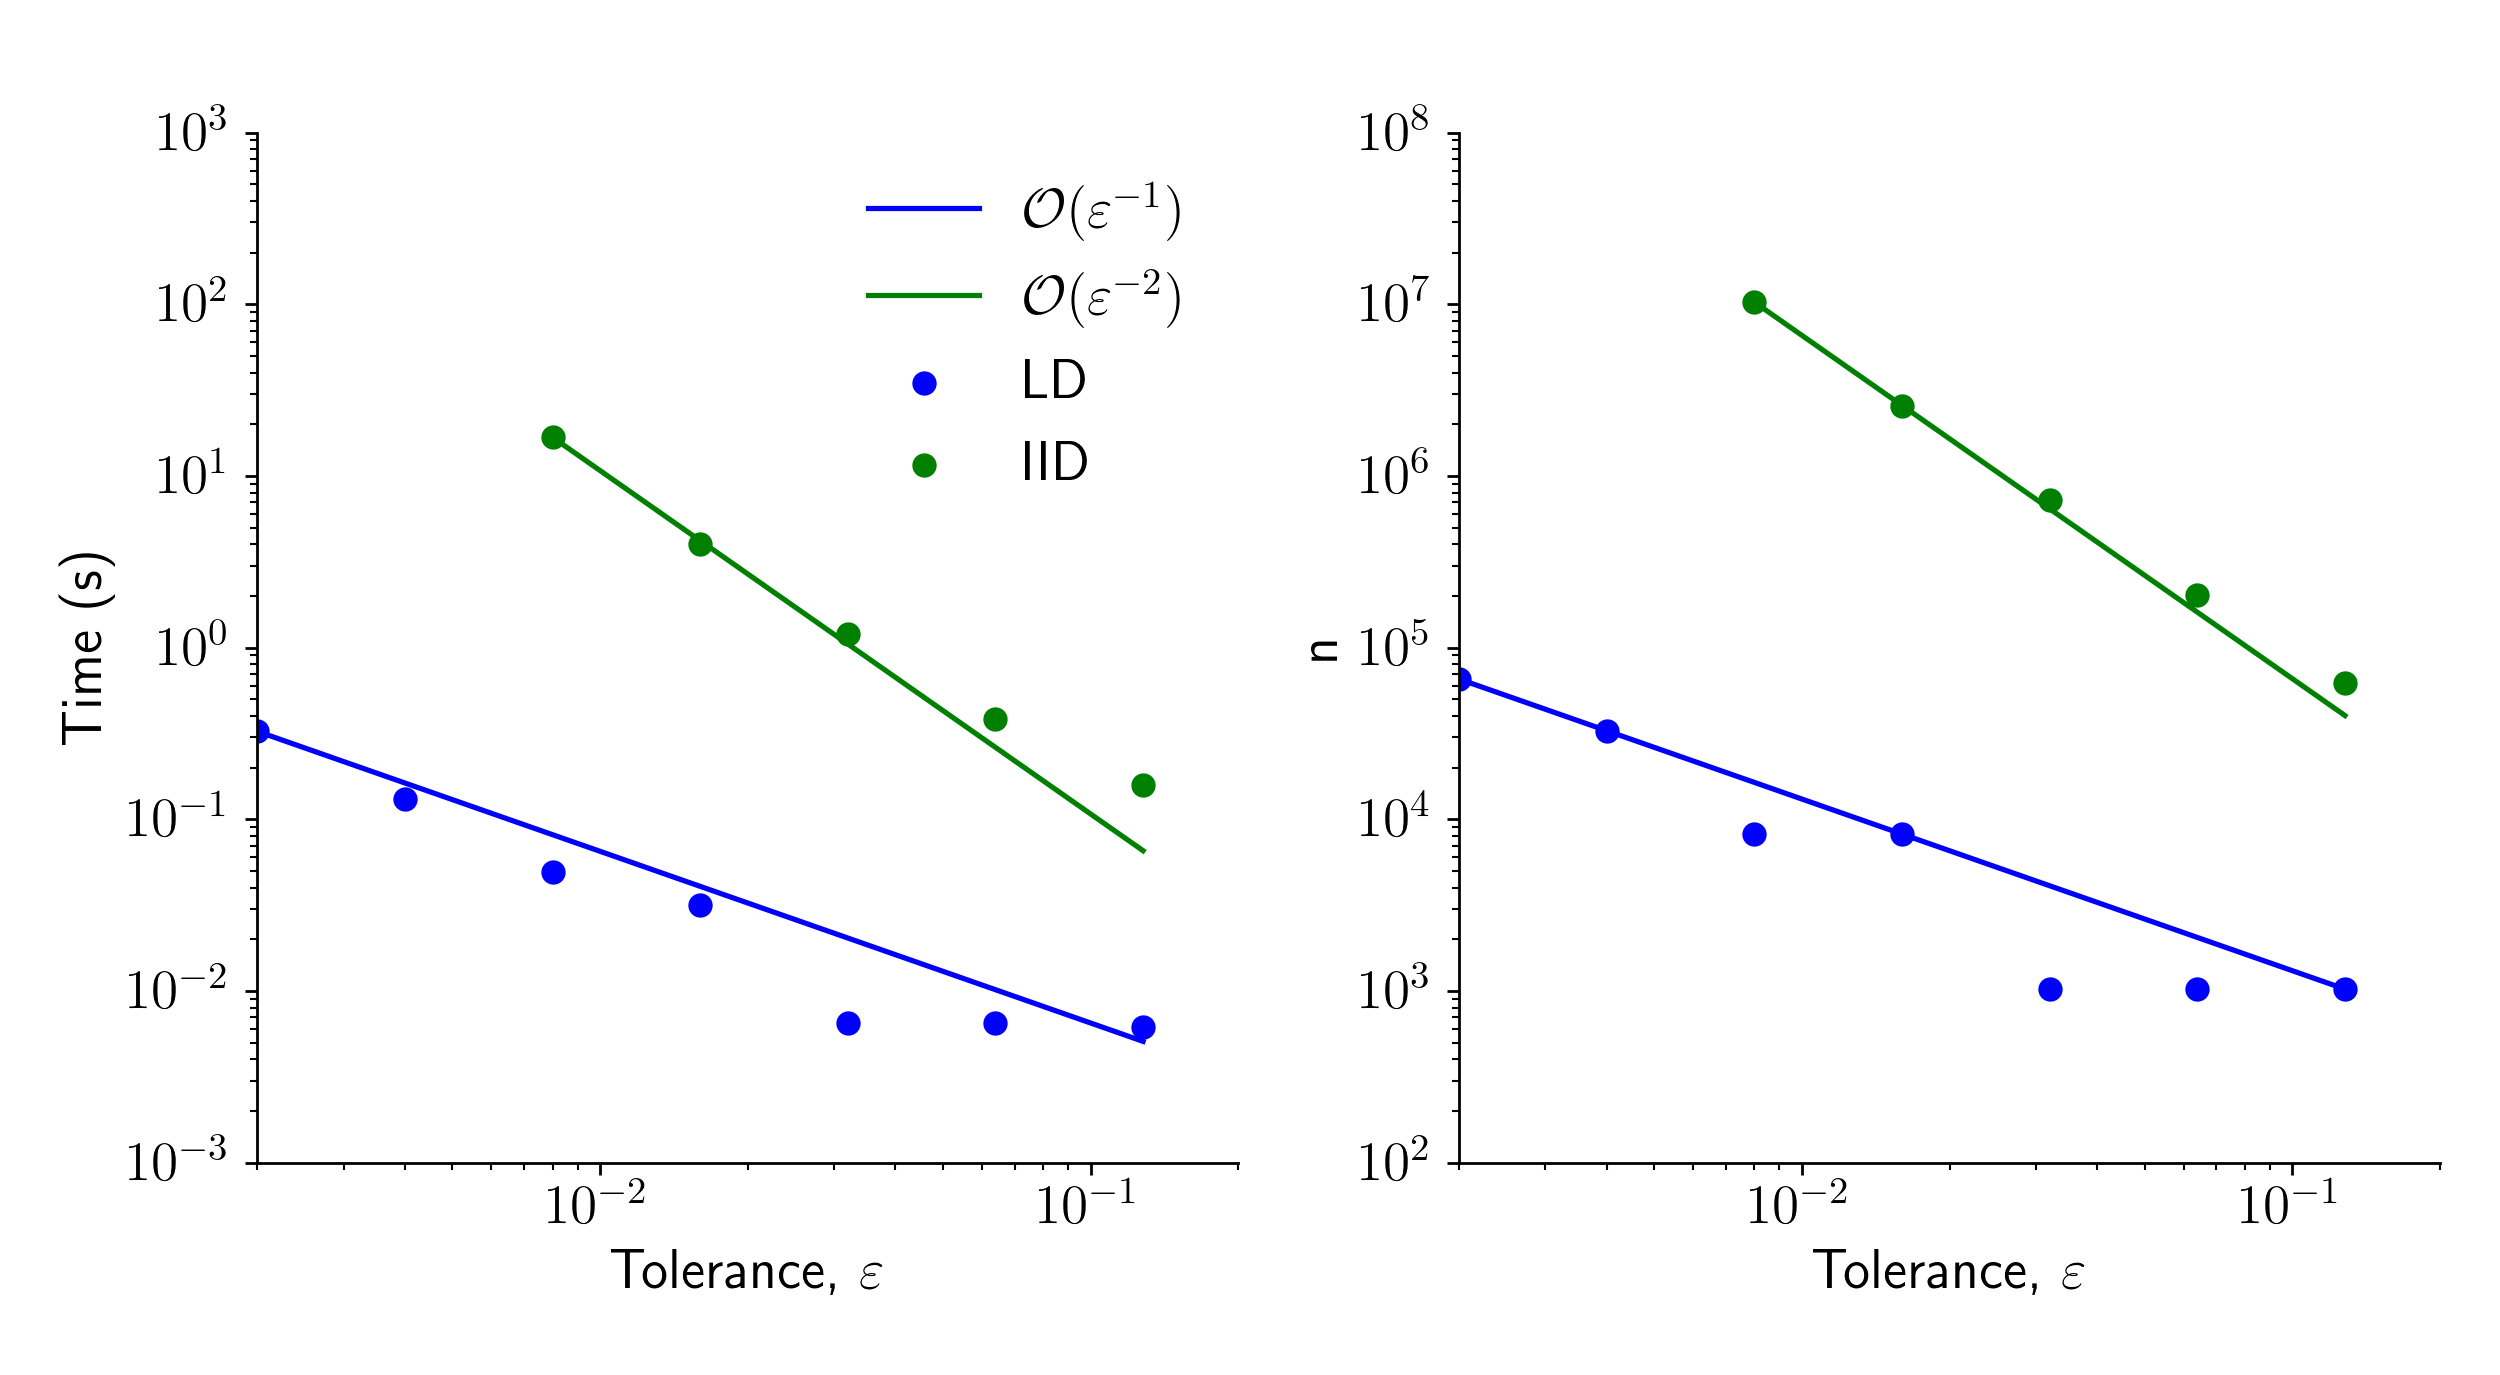
\includegraphics[height=6cm]{QMCSoftwareArticle/figs/sc_comp.png}
	\caption{Comparison of run times and sample sizes for computing the $5$-dimensional Keister integral \eqref{eq:KeisterIntegral} using IID and LD lattice sequences for a variety of absolute error tolerances.  The respective stopping criteria are  \texttt{CubMCG} \AGSComment{CITE} and  \texttt{CubQMCLatticeG} \AGSComment{CITE}. The LD sequences provide the desired answer much more efficiently.}
	\label{fig:sc_comp}
\end{figure}

For another illustration of QMC cubature, we turn to pricing an Asian arithmetic mean call option. The payoff of this option is the positive difference between the strike price averaged over the time horizon and the strike price, $K$:
$$
\text{payoff}(\bsS) = \max\left(\frac{1}{2d}\sum_{j=1}^d (S_{j-1}+S_j)-K,0\right), \quad \bsS = (S_0, \ldots, S_d).
$$
where $S_j$ denotes the stock price at time $\tau j/d$.  A basic model for stock prices is a geometric Brownian motion,
\[
S_j(\bsT) = S_0 \exp((r - \sigma^2) \tau j/d + \sigma T_j),   \;  j = 1, \ldots, d, \; \bsT = (T_1, \ldots, T_d)\sim \calN(0,\mSigma),
\]
where $\mSigma$ is defined in \eqref{eq:BMcov}, $r$ is the interest rate, $\sigma$ is the volatility, and $S_0$ is the initial price.  The fair price of the option is then the expected value of the discounted payoff, namely,
\begin{equation*}
	\text{price} = \mu = \bbE[g(\bsT)], \quad \text{where } g(\bst) = \text{payoff}\bigl(\bsS(\bst) \bigr) \exp(-r \tau).
\end{equation*}

The following code utilizes QMCPy's Asian option \texttt{Integrand} object to approximate the Asian call option for a particular choice of the parameters.
\lstinputlisting[style=Python]{QMCSoftwareArticle/python/sc_aco.txt}
Because this \texttt{Integrand} object has the built-in Brownian motion \texttt{TrueMeasure}, one only neeed provide the LD sampler.

Out of the money option price calculations can be sped up by adding a drift to the Brownian motion that produces more in the money paths.  This is a form of importance sampling.  Using a Brownian motion without drift we get
\lstinputlisting[style=Python]{QMCSoftwareArticle/python/wo_imp_samp_aco.txt}
Adding the drift gives us the answer faster:
\lstinputlisting[style=Python]{QMCSoftwareArticle/python/w_imp_samp_aco.txt}
The choice of a good drift is an art.

The improvement in time is less than improvement in $n$ because the integrand $f$ is more expensive to compute when the drift is added.  In the case of no drift, the $\lambda$ in \eqref{eq:transVar} corresponds to the density for the discrete Brownian motion, and the variable transformation $\bsPsi$ is chosen so that $\lambda\bigl(\bsPsi(\cdot)\bigr) \QMCPYabs{\partial \bsPsi/\partial \bsx} = \varrho(\bsx) = 1$ and $f(\bsx) = g\left(\bsPsi(\bsx) \right)$.  However, if we choose $\lambda_{\IMP}$ as our importance sampling density and $\bsPsi_{\IMP}$ as the variable transformation corresponding to $\lambda_\IMP\bigl(\bsPsi_\IMP(\cdot)\bigr) \QMCPYabs{\partial \bsPsi_\IMP/\partial \bsx} = \varrho(\bsx) = 1$, then
\begin{align}
	\nonumber
	\mu &= \int_\calT g(\bst) \, \lambda(\bst) \, \D \bst  = \int_\calT g(\bst) \, \frac{\lambda(\bst)}{\lambda_\IMP(\bst) } \, \lambda_\IMP(\bst) \D \bst  \\
	\nonumber
	& =  \int_\calX g\bigl(\bsPsi_\IMP(\bsx)\bigr) \, \frac{\lambda\bigl(\bsPsi_\IMP(\bsx)\bigr)} {\lambda_\IMP\bigl(\bsPsi_\IMP(\bsx)\bigr) } \lambda_\IMP\bigl(\bsPsi_\IMP(\bsx)\bigr) \,\QMCPYabs{\frac{\partial \bsPsi_\IMP}{\partial \bsx}} \, \D \bsx \\
	\nonumber
	& =  \int_\calX f_\IMP(\bsx) \, \varrho(\bsx) \, \D \bsx  \\
	\label{eq:transVarImp}
	& \qquad \qquad \text{where } f_\IMP(\bsx)  = g\bigl(\bsPsi_\IMP(\bsx)\bigr)  \,  \frac{\lambda\bigl(\bsPsi_\IMP(\bsx)\bigr)} {\lambda_\IMP\bigl(\bsPsi_\IMP(\bsx)\bigr) }
\end{align}


\begin{figure}
	\centering
	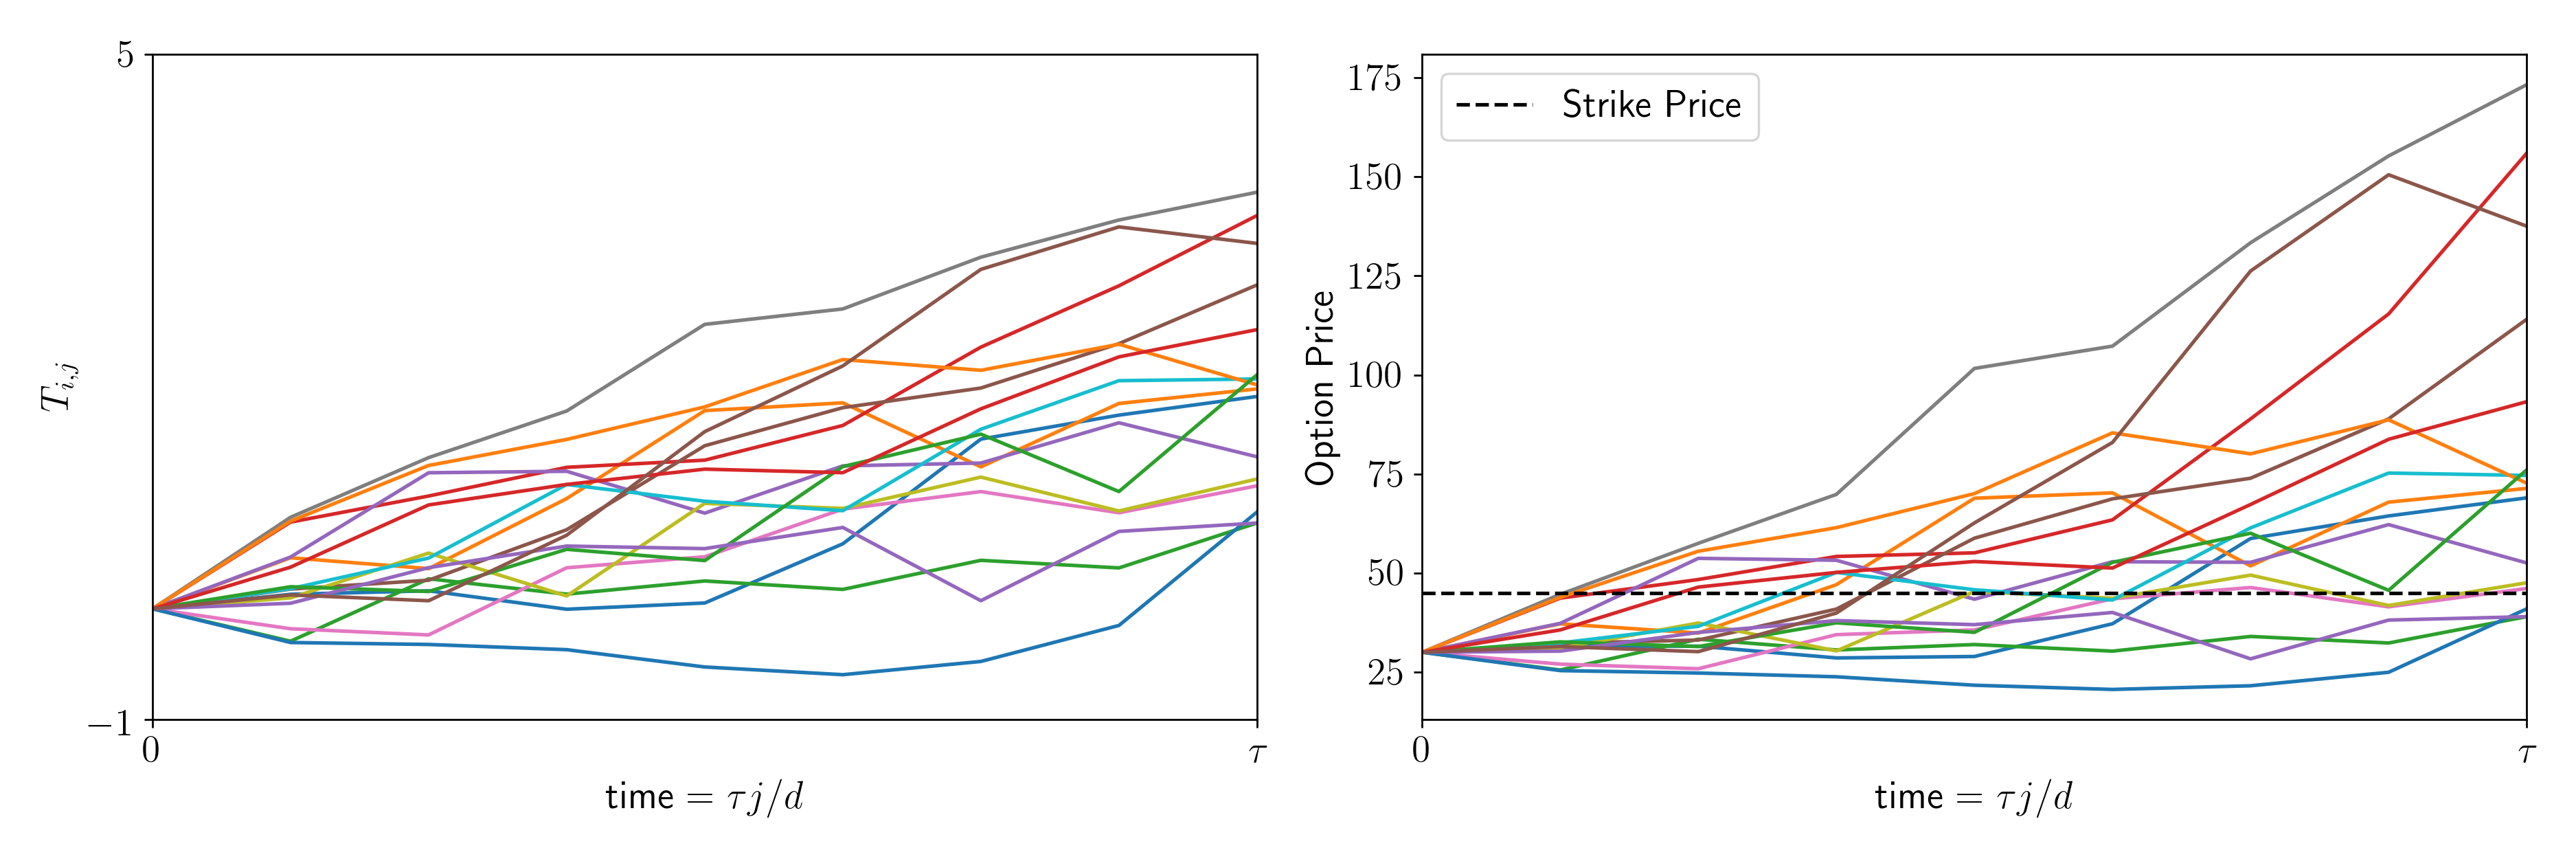
\includegraphics[width=1\textwidth]{QMCSoftwareArticle/figs/i_aco.png}
	\caption{Left: Brownian Motion paths with drift $a=2$. Right: Corresponding Asian Call option paths with $S_0=30$, $K=45$, $\sigma=0.5$, and $r=0$.}
	\label{fig:aco}
\end{figure}

Figure \ref{fig:aco} shows drifted Brownian motion paths and their corresponding option pricing paths.
\AGSComment{Bayesian stopping criterion}

\section{Under the Hood}

In this section, we look at the inner workings of QMCPy and points out available features we hope will benefit the community of QMC researchers and practitioners. We also highlight important idiosyncrasies of QMC methods and how QMCPy addresses these challenges.

\subsection{Link to LatNetBuilder}

QMCPy provides users access to high quality lattice and digital net generators (defined in Table \ref{tab:GroupProp}). A low-discrepancy generator is comprised of two parts: the static generating vectors $\bsZ_1,\bsZ_2,\bsZ_4, \dots \in [0,1)^d$ and the callable generator function. QMCPy integrates nicely with latnetbuilder \AGSComment{CITE}, a package centered around search algorithms to find high quality generating vectors. QMCPy's lattice and digital net generators can accept a vectors from latnetbuilder and use them to generate custom ordinary lattice, polynomial lattice, polynomial net, or digital net sequence. We defer readers to latnetbuilder and QMCPy documentation \AGSComment{CITE BOTH} for details.

\subsection{Customization Options for Low Discrepancy Generators}

QMCPy's low discrepancy generator routines also support numerous customizations for users who need specific points sets, orders, or randomizations. For example, our in-house developed digital net generator allows randomizations such as digital shifts and linear matrix scrambles, optional graycode orderings, and an optionally non-zero starting dimension. Moreover, while most lattice and digital net generators use a fixed generating vector, QMCPy allows users to input their own vector for their specific need, as detailed in the previous subsection.

\subsection{Preferred sample sizes for low-discrepancy generators and}

Low-discrepancy sequences differ from IID node sets in that they fill the domain in a more uniform manner. As IID nodes are independent, they do not have a preferred sample size. That is, if $\bsX \IIDsim \calU[0,1]^d$ then each node is equally likely to fall  anywhere in the unit cube. On the other hand, low-discrepancy sequences provide guarantees that the integration domain is more evenly sampled. However, these guarantees only occur at specific sample sizes. For example, lattice and digital net sequences only fill the domain evenly when $n$ is a power of $2$.

\subsection{\texttt{print}ing  QMCPy Instances}

A helpful features of QMCPy is the ability to print out components instances to see more detailed information. This allows users to quickly see the properties that have been set and defaulted for any given component. This feature was already used to print the data object returned by the stopping criterion's \texttt{integrate} method in Section \ref{CDHJS_sec:stopping_crit}. The following code prints a drifted \texttt{BrownianMotion} instance and displays the connection to an underlying Gaussian measure.
\lstinputlisting[style=Python]{QMCSoftwareArticle/python/print_bm.txt}


\AGSComment{
\begin{itemize}
    \item we have better generating vector (under latnetbuilder sub-section)
    \item transform from low discrepancy does not guarantee low discrepancy in new distribution
    \item Sobol' samples will repeat after $2^{32}$ samples
    \item multi-level stopping criterion
    \item PCA and Cholesky decomposition for Gaussian (and Brownian Motion which is a subclass of Gaussian)
\end{itemize}}

\section{Further Work} \label{CDHJS_sec:further}

\AGSComment{
\begin{itemize}
    \item Better multi-level stopping criterion (Pieterjan)
    \item Multi-composed transforms $\bsPsi$ (multiple Jacobian factors)
    \item Niederreiter sequences (Adrian and Onyekachi)
    \item Sobol' indicies (Chris Hoyt)
    \item transformations for discrete distributions that do not mimic $\calU[0,1]^d$
    \item control variates
    \item vectorized integrals
\end{itemize}}

\begin{acknowledgement}
The authors would like to thank the organizers for a wonderful MCQMC 2020.
We also thank the referees for their many helpful suggestions.  This work is supported in part by National Science Foundation grants DMS-1522687 and SigOpt.
\end{acknowledgement}

%\section*{References}
%\nocite{*}
\bibliographystyle{spmpsci.bst}
\bibliography{FJH23,FJHown23,QMCSoftwareArticle}



\AGSComment{

\section{Extra Derivations}

\subsection{Importance sampling with Gaussian}

$$ \bsPsi(\bsx) = A\Phi^{-1}(\bsx) + \mu \quad \text{where} \quad \Sigma = AA^T$$
$$ \left\lvert \frac{\D \bsPsi}{\D \bsx} \right\rvert = \det(J) \quad \text{for} \quad J_{ij} = \frac{\D \Psi_i}{\D x_j} = \frac{A_{ij}}{\phi(\Phi^{-1}(x_j))}$$
$$ \det(J) = \det\left(A . \text{diag}\left(\frac{1}{\phi(\Phi^{-1}(\bsx))}\right)\right) = \frac{\det(A)}{\prod_{j=1}^d \phi(\Phi^{-1}(x_j))}$$}

\FJHComment{Given $g$ and $\lambda$ to define your integral, suppose that $\lambda(\bst)$ is some multiple of some multivariate normal distribution:
	\begin{equation*}
		\lambda(\bst)  = \frac{c \exp\bigl(-(\bst -\bsb)^T \mLambda^{-1}(\bst -\bsb)/2\bigr)}{\sqrt{ (2\pi)^d \det(\mLambda)}}
	\end{equation*}
Suppose that we use the variable transformation $\bsPsi$ defined in \eqref{eq:exampleVarTransGauss}.  By what you have derived above:
\begin{align*}
	\QMCPYabs{\frac{\partial \bsPsi}{\partial \bsx}}
	& = \frac{\det(\mA^T)}{\prod_{j=1}^d \phi(\Phi^{-1}(x_j))} = \sqrt{(2\pi)^d \det(\mSigma)} \exp\bigl( \QMCPYnormnorm[2]{\bsPhi^{-1}(\bsx)}^2/2\bigr) \\
	\MoveEqLeft[2]{\lambda\bigl(\bsPsi(\bsx)\bigr) \QMCPYabs{\frac{\partial \bsPsi}{\partial \bsx}}} \\
	& =  c \sqrt{\frac{\det(\mSigma)}{\det(\mLambda)}} \exp \bigl( [ \bsPhi^{-1}(\bsx)^T \bsPhi^{-1}(\bsx) \\
	& \qquad \qquad -   (\mA\bsPhi^{-1}(\bsx) +\bsa -\bsb)^T\mLambda^{-1}(\mA\bsPhi^{-1}(\bsx) +\bsa -\bsb)        ] /2   \bigr) \\
	& =  c \sqrt{\frac{\det(\mSigma)}{\det(\mLambda)}} \exp \bigl( [ \bsPhi^{-1}(\bsx)^T \bsPhi^{-1}(\bsx)
	-   \bsPhi^{-1}(\bsx)^T\mA^T\mLambda^{-1}\mA \bsPhi^{-1}(\bsx)\\
	& \qquad \qquad  - 2(\bsa -\bsb)^T \mLambda^{-1}\mA\bsPhi^{-1}(\bsx) - (\bsa -\bsb)^T \mLambda^{-1} (\bsa -\bsb)] /2   \bigr)
\end{align*}
If $\mLambda = \mSigma$, then this simplifies to
\begin{equation*}
		\lambda\bigl(\bsPsi(\bsx)\bigr) \QMCPYabs{\frac{\partial \bsPsi}{\partial \bsx}}
	 =  c \exp \bigl( - (\bsa -\bsb)^T \mA^{-T} [
	2 \bsPhi^{-1}(\bsx) + \mA^{-1}(\bsa -\bsb)] /2   \bigr) .
\end{equation*}
If $\mLambda = \lambda^2 \mI$ and  $\mA = \sigma \mI$, then
\begin{align*}
	\lambda\bigl(\bsPsi(\bsx)\bigr) \QMCPYabs{\frac{\partial \bsPsi}{\partial \bsx}}
	& = \frac{c\sigma}{\lambda}
	\exp \bigl( [ (\lambda^2 -\sigma^2)\bsPhi^{-1}(\bsx)^T\bsPhi^{-1}(\bsx)
	\\
	& -  (\bsa -\bsb)^T [
	2\sigma \bsPhi^{-1}(\bsx) + (\bsa -\bsb)] /(2\lambda^2)   \bigr) .
\end{align*}
}

\AGSComment{

\subsection{Chaining Transforms}
With $k$ transforms, let $\hat{\bsPsi}_j(\bsx) = (\bsPsi_j \circ \bsPsi_{j-1} \circ \dots \circ \bsPsi_1)(\bsx)$ denote the first $j$ compositions and $\bst = \hat{\bsPsi}_k(\bsx)$ be the complete transformation. Then,
$$f(\bsx) = g(\hat{\bsPsi}_k(\bsx)) \frac{\lambda(\hat{\bsPsi}_k(\bsx))}{\varrho(\bsx)} \prod_{i=1}^{k} \left\lvert \frac{\D \, \bsPsi_i}{\D \, \hat{\bsPsi}_{i-1}(\bsx)} \right\rvert$$
where $\hat{\bsPsi}_0(\bsx) = \bsx$.
}

\FJHComment{

\subsection{Software Framework}

\newcommand{\dd}{\texttt{DiscreteDistribution}\xspace}
\newcommand{\tm}{\texttt{TrueMeasure}\xspace}

\begin{itemize}
\item \dd $\rightarrow$ \tm gives an instance that can generate a sequence that mimics the measure specified by \tm if \tm is a probability measure; it also has a \texttt{gen\_samples} method.

\item if \tm is not a probability measure, then \dd $\rightarrow$ \tm sets up a transformation from $\calX$ to $\calT$.

\item \texttt{CustomFun} takes a user-defined function $g$ and a \tm instance and uses the $\lambda$ inferred from the \tm to form $f$.

\item Built-in \texttt{Integrand} classes know what $g$ and $f$ are.

\begin{itemize}
    \item One way is to have these \texttt{Integrand} classes assume a \tm and only need a \dd input. If you do not like the default \tm, then you need to input your own.

    \item Another way is to have these \texttt{Integrand} classes take a \tm input and use that, plus their knowledge of $g$ and $\lambda$ to find $f$, perhaps by what could be considered importance sampling.

\end{itemize}
\end{itemize}
}

\end{document}





\section{Tenets of Great Software} \label{CDHJS_sec:tenets_of_great_software}

In this section we lay out common aspirations of scientific software. While some objectives are expected by practitioners, e.g. correctly written software, others may better be characterized as features that are pursued as a project matures, e.g. supporting scalable computation. The following paragraphs highlight aspirations with more important, expected behaviours coming earlier in the discussion.

Software is expected to be \emph{correct}. A practitioner generating a digital sequence expects the routine to produce theoretically accurate points. For example, the QMC community has helped developers ensure implementations of low discrepancy sequence generators include the zeroth point \cite{Owe22a, scipySobol2020a} and  have correct randomization routines. %, and disallow thinning / leaping: taking every $k^\text{th}$ value in the sequence.

Algorithms should be implemented in an \emph{efficient} manner. Both the compute time and memory requirements should match theoretical developments which in turn should be as close to the state of the art as possible. As a classical example, it is expected that an implementation of the discrete Fourier transform for $n$ points has complexity $\mathcal{O}(n\log n)$.

Software should be \emph{accessible} in terms of installation, presentation, navigation, exemplification, and communication. A library should be straightforward to install from a common distribution platform, consistent in user interface, intuitive to navigate to modules and documentation, comprehensible in its' examples, and supportive in user engagement. Software accessibility considerations are further discussed in Sect.\ \ref{CDHJS_sec:language_library_environment}.

Libraries should be \emph{sustainable} for future development. The goal should be to have a sufficient user base and developer community for updates and maintenance. Similar to accessibility, sustainability is often overlooked for aspirations discussed later in this section. However, we contend that a sub-optimal but user-friendly library with community engagement may be more impactful than an optimal library which lacks support. We promote collaborative, community driven development further in Sect.\ \ref{CDHJS_sec:encouraging_collaborative_developement}.

Software should be \emph{integrated} into the environment's scientific software ecosystem. More simply, libraries should play nicely together and utilize the mature developments of other teams. A simple example in \AGSComment{CITE} shows a straightforward integration between the QMC package QMCPy \cite{QMCPy2020a} and the PDE package FEniCS/Dolfin \cite{LoggEtal_10_2012}, both in Python.

Routines should be \emph{scalable} to advanced computer architectures. The widespread availability of on demand computing with multi-core and multi-GPU machines encourages software that can take advantage of parallel computation. Scalable algorithms lend themselves to a larger class or problems and provide practitioners the opportunity to more quickly test ideas.

\section{(Quasi-)Monte Carlo Software Architecture} \label{CDHJS_sec:qmc_software_architecture}

An important step in the development of any software is to determine its' architecture. How should components interact with each other? Which aspects should be modular? Object oriented? Procedural? Answers to these questions form the blueprint of software design and guide implementation.

This section proposes an object oriented design for (Q)MC software. The authors have implemented this architecture into the QMCPy \cite{QMCPy2020a} Python package which is further detailed in the MCQMC 2020 proceedings article \AGSComment{CITE}. While this is not the only possible architecture for (Q)MC problems, we hope the high level object definitions facilitate easy collaboration and integration for research across the (Q)MC community.

The standard (Q)MC problem is to approximate the true mean $\mu := \mathbb{E}[g(\boldsymbol{T})]$ where $\boldsymbol{T}$ is some $d$ dimensional random variable. For nice $\boldsymbol{T}$, one may perform a change of variables to write $\mu = \mathbb{E}[f(\boldsymbol{X})]$ where $\boldsymbol{X} \sim \mathcal{U}[0,1]^d$. For example, if $\boldsymbol{T} \sim \mathcal{N}(\boldsymbol{0},\boldsymbol{I})$, then one may set $f(\boldsymbol{x}) := g(\boldsymbol{\Phi}^{-1}(\boldsymbol{x}))$ for $\boldsymbol{x} \in [0,1]^d$ where $\boldsymbol{\Phi}^{-1}$ is the inverse CDF of a standard normal distribution taken element wise. One may then approximate $\mu$ by the $n$ sample average $\hat{\mu} = 1/n \sum_{i=1}^n f(\boldsymbol{x}_i)$ where $\{\boldsymbol{x}_i\}_{i=1}^n$ are chosen so their empirical distribution is ``close'' to the uniform distribution. The approximation error $\varepsilon = \lvert \mu - \hat{\mu} \rvert$ is $\mathcal{O}(n^{-1/2})$ when $\{\boldsymbol{x}_i\}_{i=1}^n$ are chosen to be IID standard uniform as in the case of simple Monte Carlo (MC) and almost $\mathcal{O}(n^{-1})$ when $\{\boldsymbol{x}_i\}_{i=1}^n$ are chosen from a low discrepancy sequence as done for Quasi-Monte Carlo (QMC). Instead of selecting the number of samples $n$ and then determining the error $\varepsilon$, it is often desirable to select $\varepsilon$ and then adaptively determine $n$. From this view, $n$ is $\mathcal{O}(\varepsilon^{-2})$ for MC and almost $\mathcal{O}(\varepsilon^{-1})$ for QMC. A more detailed account of MC and QMC can be found in \AGSComment{CITE}.

The (Q)MC pipeline above can be decomposed into $4$ main components:
\begin{description}
    \item[\textbf{Generator:}] producing $\{\boldsymbol{x}_i\}_{i=1}^n$ whose empirical distribution is ``close'' to the standard uniform distribution in $d$ dimensions for any $n \geq 1$.  May produce IID or low discrepancy sequences depending on the problem.
    \item[\textbf{Measure:}] that defines the distribution of $\boldsymbol{T}$ e.g., uniform, Gaussian, Lebesgue. This definition facilitates choosing a change of variables to determine $f$.
    \item[\textbf{Integrand:}] $g$, which defines the original integral. When provided knowledge of the true measure, the integrand can also evaluate $f$ via the change of variables.
    \item[\textbf{Stopping Criterion:}] based on a data-driven error bound, which determines how large $n$ should be to ensure that $\varepsilon$ is less than some user-provided error threshold.
\end{description}
A variety of QMC materials and the their categorizations into the above framework are described in the following list.
\begin{itemize}
    %\item \cite{LEc2017a} provides a history of random number generation
    %\item Notorious RANDU from the 1960s \cite{RANDU}, which fails the spectral test
    %\item VEGAS \cite{Lep78a, Lep21a} importance sampling Monte Carlo algorithm favored by physicists
    \item ACM low discrepancy point generators \cite{BraFox88,BraFoxNie92,HonHic00a}
    \item FinDer \cite{PasTra95,FinDer} and BRODA \cite{BRODA20a} targeting quantitative finance
    \item Korobov cubature and scrambled Sobol' generators in NAG \cite{NAG27} for decades
    \item Scrambled Sobol' and Halton generators in MATLAB \cite{MAT9.13} since 2008, and fixed a few years later
    %\item BUGS \cite{BUGSBook, BUGSweb} and Stan \cite{STAN} for Markov Chain Monte Carlo (MCMC)
    \item LatMRG \cite{LEcCou97}, RNGStreams \cite{LEcEtal02},  SSJ \cite{LEc2002a,SSJ}, and LatNetBuilder \cite{LatNet}
    \item Low discrepancy generators \cite{FriKel02,FriKelweb}, SamplePack \cite{SamplePack}, \cite{GruWeb},  and MatBuilder \cite{paulin2022}
    \item Sobol' direction numbers \cite{JoeKuo03,JoeKuo08,SobolDirection}
    \item Fast CBC, Magic Point Shop, QMC4PDE and other code since 2004  at \cite{NuyWeb}
    \item Multi-level software \cite{GilesSoft,GilesQSoft}
    \item Data-driven error bounds and stopping criteria in GAIL \cite{ChoEtal21a} and QMCPy \cite{QMCPy2020a, ChoEtal22a}
    \item Uncertainty quantification libraries Dakota \cite{DakotaUsersManual}, UQTk \cite{DebEtal04,UQTk}, and MUQ \cite{MUQ}  have some basic level low discrepancy sampling
    \item QMC framework in Julia since 2019 \cite{QMCJulia} by Robbe and others
    \item Scrambled Sobol' in SciPy \cite{virtanen2020scipy} and PyTorch \cite{paszke2019pytorch} since several years ago
    \item TensorFlow QMC framework \cite{tfqfQMC2021a} since a year or so ago
    \item CUBA \cite{CUBA}
\end{itemize}

\section{Choosing a Environment} \label{CDHJS_sec:language_library_environment}

This section discusses the challenges in choosing environments for development and distribution. The development environment includes the choice of which languages, architectures, testing methods, and documentation methods to support. The deployment environment will often be influenced by the choice of programming languages.

The choice of programming language should be aligned with the communities the team wishes to reach with their software. The choice should also account for developer familiarity and ability to quickly prototype ideas. A team should align their choice of language to balance the desire to have user-friendly prototyping code versus the desire to have high performance computing (HPC) ``ninja'' code written for production setting. To the second point, it is also important to consider which language will best facilitate the parallel and GPU computations the team wishes to support.

Many programming languages come bundled with their own preferred distribution systems. Python has PyPI, R has CRAN, Julia has Pkg. However, many projects support multiple languages and have complex dependency requirements. In such cases, it can be helpful to containerize your application using a service like Docker.

\section{Encouraging Collaborative Development} \label{CDHJS_sec:encouraging_collaborative_developement}

We now discuss ways a team may encourage collaborative development while touching on a few best practices. As discussed earlier, collaborative development promotes greater community engagement, ecosystem integration, and software longevity.

The authors have found the Git version control system to be an invaluable for software development. Git hosts such as GitHub or Bitbucket may offer teams additional features such as tracking issues, managing discussion threads, and setting up automated workflows for jobs such as testing and documentation compilation.

Accessibility is key to community engagment. It is paramount that your package be easy to install, well documented, and tested regularly. Aside from static communications, a team should also be engaged in addressing users bugs and be attentive to collaborating with proposed code changes.

It is also important for a development team to make a clear path for collaborators to contributors to the software. Templates for issues and pull requests are a good place to start. Contributors should also be encouraged to write robust tests for their updates and highlight their new features in a demo for greater accessibility.

\section{Example Collaboration with UMBridge and QMCPy} \label{CDHJS_sec:example_collaboration_umbridge}

This section discusses a collaboration between the UM-Bridge (the UQ and Model Bridge) \AGSComment{CITE} and QMCPy (the Quasi-Monte Carlo Python library) \cite{QMCPy2020a} softwares. The UM-Bridge documentation describes its' mission is to, ``provide a unified interface for numerical models that is accessible from virtually any programming language or framework. It is primarily intended for coupling advanced models (e.g. simulations of complex physical processes) to advanced statistics or optimization methods.'' QMCPy is a high level framework for combining QMC components in a compatible and consistent manner. The collaboration between these two packages focused on making the UQ methods of QMCPy compatible with the abstract model representations from UM-Bridge. Specifically, UM-Bridge models are made compatible with the QMCPy framework through an integrand wrapper for seamless compatibility with a variety of existing point generators, transformations, and stopping criterion already available in QMCPy.

To exemplify the integration, we focus on quantifying uncertainty propagation of material properties of a cantilevered beam. It is assumed the beam is split into $3$ regions of random stiffness dependent on uncertain material properties. Given a sample of $3$ stiffness values, the UM-Bridge model provides the displacement at $31$ equidistant nodes along the beam. Our task is to quantify the uncertainty in displacement at each of these $31$ locations along the beam.

A fully coded example of this problem is available at \url{https://github.com/QMCSoftware/QMCSoftware/blob/master/demos/umbridge.ipynb}. At a high level, one begins by running the UM-Bridge model in a Docker container. A model is then initialized in the UM-Bridge Python client which is then provided to QMCPy alongside a low discrepancy point generator and distribution governing the $3$ beam stiffness values. QMCPy then performs adaptive QMC cubature to simultaneously approximate the expected displacement at the $31$ locations of interest. When the cubature method queries the model, the QMCPy wrapper around UM-Bridge model sends requests to the Docker UM-Bridge model in parallel. The load balancing provided by UM-Bridge may be utilized to evaluate the model in parallel, a potentially advantageous feature for models which are costly to evaluate. Figure \ref{fig:umbridge_muq} depicts the $31$ approximate expected displacement values subject to uniform stiffness.

\begin{figure}
    \centering
    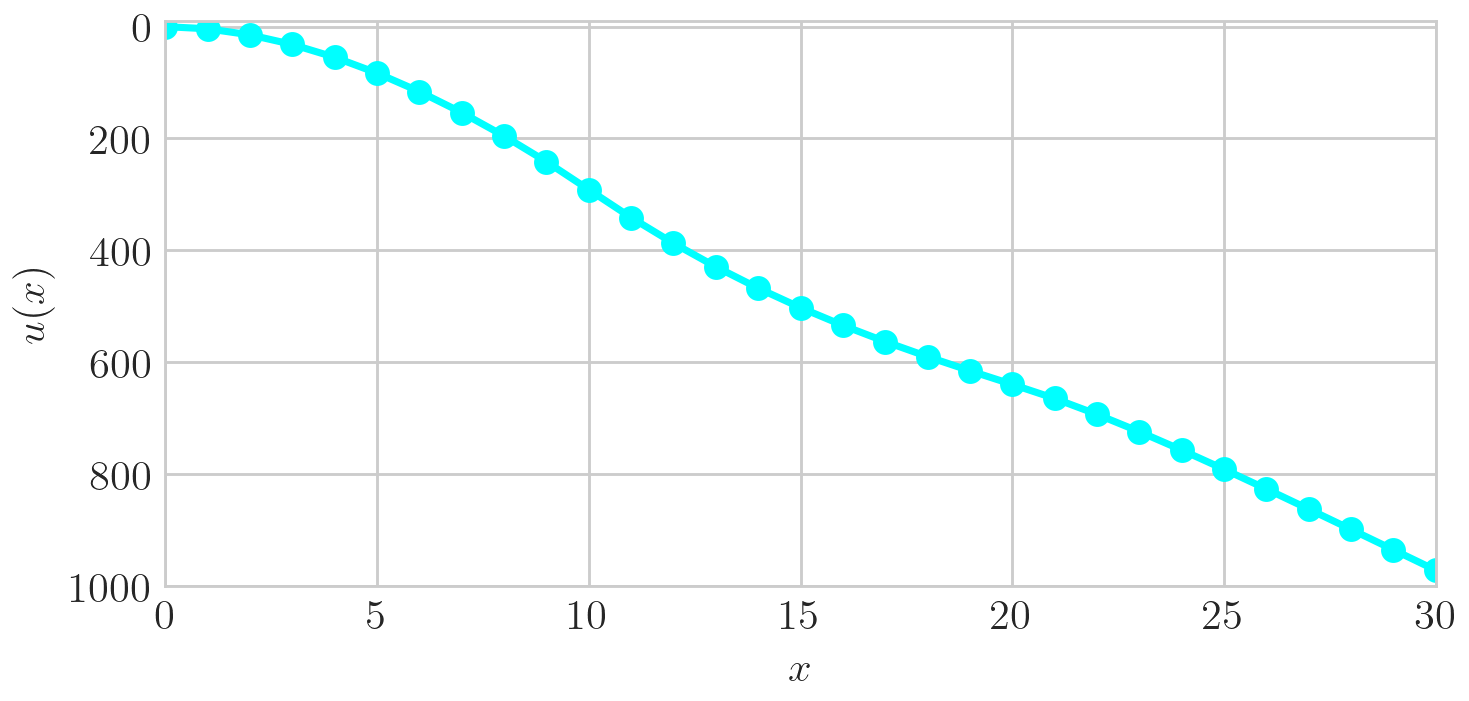
\includegraphics[height=4cm]{umbridge_muq.png}
    \caption{QMCPy approximate expected displacement at $31$ locations subject to random uniform stiffness. }
    \label{fig:umbridge_muq}
\end{figure}

\section*{TODO}
\begin{itemize}
    \item Flesh out Section \ref{CDHJS_sec:encouraging_collaborative_developement}
    \item QMC Software Architecture section: better way then description of components and list of softwares?
    \item For Section \ref{CDHJS_sec:tenets_of_great_software}, the slides also include
    \begin{itemize}
        \item  Complete---contain the components or  easily access components in other libraries to solve real, complex problems
        \item Current---include the latest and best algorithms
    \end{itemize}
    which I think fall under the umbrella of software being \emph{integrated} with the community.
    \item update QMCPy citation \cite{QMCPy2020a}
    \item figures?
    \item I have left out or been breif about material from the following slides: QMCPy + FEniCS/Dolfin,  Building a Developer Team for Your Library
\end{itemize}



Developing software to implement such enhanced MC strategies poses a number of challenges. First, a development team must determine the value of the software to the users. We discuss why great (Q)MC software in necessary in Sect.\ \ref{CDHJS_sec:why_we_need_software}. Second, a team must determine high level objectives for the software; the tenets of great software are described in Sect.\ \ref{CDHJS_sec:tenets_of_great_software}. Third, an architecture for the  (Q)MC software should be determined. We propose a modularization of the (Q)MC pipeline in Sect.\ \ref{CDHJS_sec:qmc_software_architecture}. Next, a team must choose which programming languages, hardware environments, and distribution platforms they wish to support. We discuss the nuance and challenges in these decisions in Sect.\ \ref{CDHJS_sec:language_library_environment}. Finally, a project which hopes to stand the test of time must draw attention and support from the broader (Q)MC community. To this end, we encourage collaborative community development and describe its' best practices in  Sect.\ \ref{CDHJS_sec:encouraging_collaborative_developement}.